\documentclass[supercite]{Experimental_Report}

\title{~~~~~~数据结构实验~~~~~~}
\author{郭凯锐}
\school{计算机科学与技术学院}
\classnum{CS2208}
\stunum{U202215595}
\instructor{袁凌} 
\date{2023年5月28日}

\usepackage{algorithm, multirow}
\usepackage{algpseudocode}
\usepackage{amsmath}
\usepackage{amsthm}
\usepackage{framed}
\usepackage{mathtools}
\usepackage{subcaption}
\usepackage{xltxtra}
\usepackage{bm}
\usepackage{tikz}
\usepackage{tikzscale}
\usepackage{pgfplots}
\usepackage{listings}

%\usepackage{enumerate}

\lstset{
 columns=flexible,       
 numbers=left,                                        % 在左侧显示行号
 numberstyle=\tiny\color{gray},                       % 设定行号格式
 frame=none,                                          % 不显示背景边框
 backgroundcolor=\color[RGB]{245,245,244},            % 设定背景颜色
 keywordstyle=\color[RGB]{40,40,255},                 % 设定关键字颜色
 numberstyle=\footnotesize\color{darkgray},           
 commentstyle=\it\color[RGB]{0,96,96},                % 设置代码注释的格式
 stringstyle=\rmfamily\slshape\color[RGB]{128,0,0},   % 设置字符串格式
 showstringspaces=false,                              % 不显示字符串中的空格
 language=c,                                        % 设置语言
}


\pgfplotsset{compat=1.16}

\newcommand{\cfig}[3]{
	\begin{figure}[htb]
		\centering
		\includegraphics[width=#2\textwidth]{images/#1.png}
		\caption{#3}
		\label{fig:#1}
	\end{figure}
}

\newcommand{\sfig}[3]{
	\begin{subfigure}[b]{#2\textwidth}
		\includegraphics[width=\textwidth]{images/#1.png}
		\caption{#3}
		\label{fig:#1}
	\end{subfigure}
}

\newcommand{\xfig}[3]{
	\begin{figure}[htb]
		\centering
		#3
		\caption{#2}
		\label{fig:#1}
	\end{figure}
}

\newcommand{\rfig}[1]{\autoref{fig:#1}}
\newcommand{\ralg}[1]{\autoref{alg:#1}}
\newcommand{\rthm}[1]{\autoref{thm:#1}}
\newcommand{\rlem}[1]{\autoref{lem:#1}}
\newcommand{\reqn}[1]{\autoref{eqn:#1}}
\newcommand{\rtbl}[1]{\autoref{tbl:#1}}

\algnewcommand\Null{\textsc{null }}
\algnewcommand\algorithmicinput{\textbf{Input:}}
\algnewcommand\Input{\item[\algorithmicinput]}
\algnewcommand\algorithmicoutput{\textbf{Output:}}
\algnewcommand\Output{\item[\algorithmicoutput]}
\algnewcommand\algorithmicbreak{\textbf{break}}
\algnewcommand\Break{\algorithmicbreak}
\algnewcommand\algorithmiccontinue{\textbf{continue}}
\algnewcommand\Continue{\algorithmiccontinue}
\algnewcommand{\LeftCom}[1]{\State $\triangleright$ #1}

\newtheorem{thm}{定理}[section]
\newtheorem{lem}{引理}[section]

\colorlet{shadecolor}{black!15}

\theoremstyle{definition}
\newtheorem{alg}{算法}[section]

\def\thmautorefname~#1\null{定理~#1~\null}
\def\lemautorefname~#1\null{引理~#1~\null}
\def\algautorefname~#1\null{算法~#1~\null}

\begin{document}

\maketitle

\clearpage

\pagenumbering{Roman}

\tableofcontents[level=2]

\clearpage

\pagenumbering{arabic}

\section{基于链式存储结构的线性表实现}

\subsection{问题描述}

\noindent 实验要求:
\begin{enumerate}
	\item 实现对链表的基本操作;
	\item 选择性实践对链表的进阶操作;
	\item 设计演示系统。
\end{enumerate}
通过实验达到:
\begin{enumerate}
	\item 加深对线性表的概念、基本运算的理解;
	\item 熟练掌握线性表的逻辑结构与物理结构的关系;
	\item 物理结构采用单链表,熟练掌握线性表的基本运算的实现。
\end{enumerate}
\subsection{系统设计}
\subsubsection{演示系统菜单的组织架构}
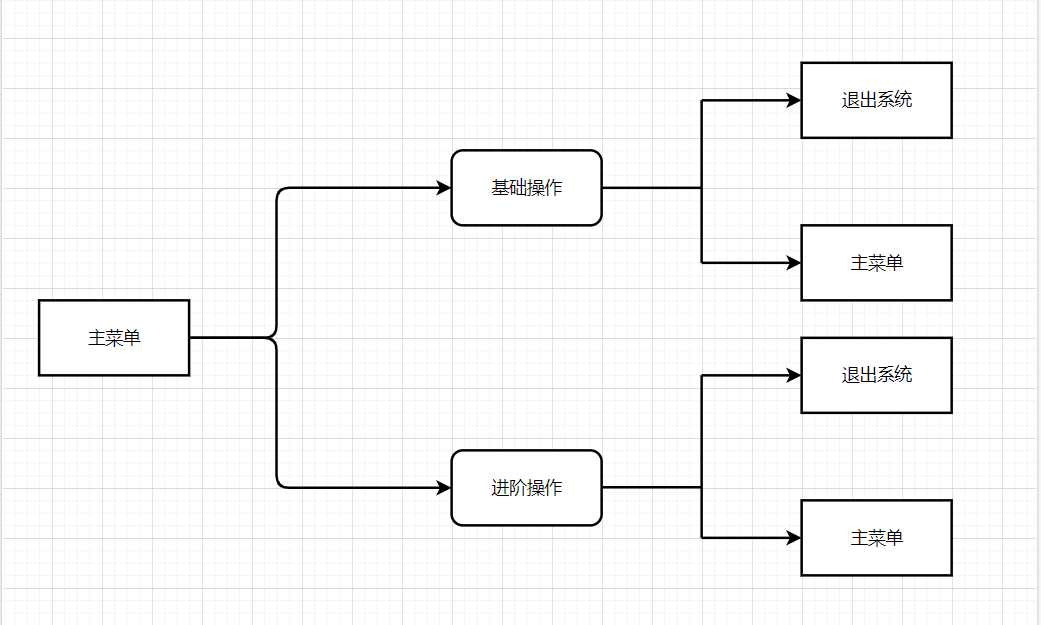
\includegraphics[width=1\linewidth]{Data_Structure/images/2.1.png}
\vspace{-0.2cm}
\clearpage
\quad 演示系统分为基本操作和进阶操作两部分,以菜单为主界面,以序号1至12表示创建,销毁,清空,插入,删除,求表长等基本操作,以序号13至17表示保存为文件,加载文件,翻转链表,对链表排序等进阶操作,以序号0表示退出演示系统,根据序号调用函数执行操作。

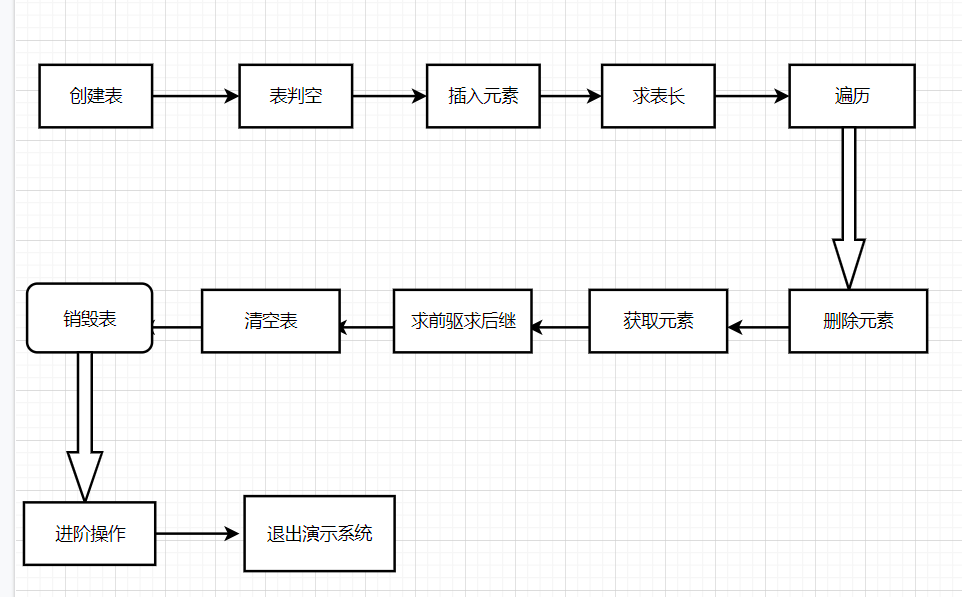
\includegraphics[width=1\linewidth]{Data_Structure/images/2.2.png}
\vspace{-0.2cm}

\clearpage
\subsubsection{ADT数据结构设计}
\noindent 对链表数据类型的定义如下:\par
\begin{lstlisting}[language=C] 
typedef int status;
typedef int ElemType; //type of element


typedef struct LNode{
	ElemType data;
	struct LNode *next;
}LNode, *LinkList;
\end{lstlisting}
对一些常量的定义如下:
\begin{lstlisting}[language=C] 
#define TRUE 1
#define FALSE 0
#define OK 1
#define ERROR 0
#define INFEASIBLE -1
#define OVERFLOW -2
#define MAX_NUM 10
#define LIST_INIT_SIZE 100
#define LISTINCREMENT  10
\end{lstlisting}

\subsubsection{初始化表}
输入:顺序表(未知状态)

输出:函数执行状态

算法的思想描述:为L结点分配存储空间,将L->next结点置空
\begin{lstlisting}{language=C}
status InitList(LinkList *L)
//initiate a list
{
	*L = (LinkList)malloc(sizeof(LNode));//malloc a node
	if(*L == NULL)
	{
		exit(OVERFLOW);//malloc failed
	}
	(*L)->data = 0;
	(*L)->next = NULL;//the list is empty
	return OK;
}
\end{lstlisting}
算法处理步骤:
\begin{enumerate}
	\renewcommand{\labelenumi}{\theenumi)}
	\item 如果顺序表L不存在,则为L分配存储空间。
	\item 如果分配成功,将L->next置空返回状态OK。
	\item 如果分配失败,返回状态 OVERFLOW 并推出该程序块。
	\item 如果顺序表存在,返回状态 INFEASIBLE 以指出无法创建。
\end{enumerate}

时间复杂度:O(1)

空间复杂度:O(1)

\subsubsection{销毁表}
输入:顺序表(未知状态)

输出:函数执行状态

算法的思想描述:用 while 循环依次释放所有节点的储存空间,再将 L 置为 NULL。

\begin{lstlisting}[language=C] 
status DestroyList(LinkList *L)
//destroy a list
{
	LinkList p, q;
	p = *L;
	while(p)
	{
		q = p->next;
		free(p);
		p = q;
	}
	*L = NULL;
	return OK;
}
\end{lstlisting}

时间复杂度:O(n)

空间复杂度:O(1)
\subsubsection{清空表}
输入:顺序表(未知状态)

输出:函数执行状态

算法的思想描述:用while循环释放除头节点以外的所有节点的储存空间,再将 L->next 置为 NULL。

\begin{lstlisting}[language=C] 
status ClearList(LinkList *L)
//clear a list
{
	LinkList p, q;
	p = (*L)->next;//point to the first node
	while(p)
	{
		q = p->next;
		free(p);
		p = q;
	}
	(*L)->next = NULL;
	return OK;
}
\end{lstlisting}

时间复杂度:O(n)

空间复杂度:O(1)
\subsubsection{表判空}
输入:顺序表(未知状态)

输出:函数执行状态

算法的思想描述:判断 L->next 是否为 NULL,若为 NULL,则链表为空,否则链表不为空。
\begin{lstlisting}[language=C] 
status ListEmpty(LinkList L)
//judge if the list is empty
{
	if(L->next)
		return FALSE;
	else
		return TRUE;
}
\end{lstlisting}

时间复杂度:O(1)

空间复杂度:O(1)
\subsubsection{求表长}

输入:顺序表L

输出:顺序表的长度

算法思想描述:遍历整个顺序表
\begin{lstlisting}
int ListLength(LinkList L)
//get the length of the list
{
	int i = 0;
	LinkList p = L->next;
	while(p)
	{
		i++;
		p = p->next;
	}
	return i;
}

\end{lstlisting}
算法处理步骤:
\begin{enumerate}
	\renewcommand{\labelenumi}{\theenumi)}
	\item 如果L存在,从头开始遍历。
	\item 若不为空则移动指针到下一个结点,长度加1。
	\item 返回长度的值。
\end{enumerate}

时间复杂度:O(n)

空间复杂度:O(1)
\subsubsection{获取元素}
输入:顺序表(未知状态)

输出:L中第i个数据元素的值e

算法的思想描述:若 i 小于 1 或大于链表的长度,则该序号非法,返回 ERROR。否则遍历至第 i 个元素,返回其数据域的值。	
\begin{lstlisting}[language=C] 
status GetElem(LinkList L, int i, ElemType *e)
//get the element of the No.i node
{
	int j = 1;
	LinkList p;
	p = L->next;
	while(p && j < i)
	{
		p = p->next;
		++j;
	}
	if(!p || j>i)
		return ERROR;
	*e = p->data;
	return OK;
}
\end{lstlisting}

时间复杂度:O(n)

空间复杂度:O(1)
\subsubsection{定位元素}
输入:顺序表(未知状态)

输出:L中第1个与e相等的元素的序号,若这样的数据元素不存在,则值为 0

算法的思想描述:声明 i=0,遍历链表查找是否有值与 e 相同的元素,每进入下一个节点时 i 自增,若找到相应元素则返回 i,否则返回 ERROR。
\begin{lstlisting}[language=C] 
int LocateElem(LinkList L, ElemType e, status(*compare)(ElemType a, ElemType b))
//get the position of the element
{
	int i = 0;
	LinkList p = L->next;
	while(p)
	{
		i++;
		if((*compare)(p->data, e))
			return i;
		p = p->next;
	}
	return 0;
}

status compare(ElemType a, ElemType b)
{
    if(a == b)
        return TRUE;
    else
        return FALSE;
}
\end{lstlisting}

时间复杂度:O(n)

空间复杂度:O(1)
\subsubsection{获得前驱}

输入:顺序表L,元素e,引用参数pre。

输出:函数的执行状态.

算法思想的描述:遍历顺序表.
\begin{lstlisting}{language=C}
status PriorElem(LinkList L, ElemType cur_e, ElemType *pre_e)
//get the element before the cur_e
{
	LinkList p = L->next;
	if(p->data==cur_e) 
		return ERROR;
	while(p->next != NULL && p->next->data != cur_e)
		p = p->next;

	if(p->next == NULL)
		return OVERFLOW;

	*pre_e = p->data;
	return OK;
}
\end{lstlisting}
算法处理步骤:
\begin{enumerate}
	\renewcommand{\labelenumi}{\theenumi)}
	\item 如果顺序表L不存在,则输出INFEASIBLE。
	\item 如果L存在,从头开始遍历。
	\item 若当前节点的后继值为e,则将当前节点的值赋给pre,输出OK。
	\item 若为找到,则返回INFEASIBLE.
\end{enumerate}

时间复杂度:O(n)

空间复杂度:O(1)
\subsubsection{求后继}
输入:顺序表(未知状态)

输出:函数执行状态

算法的思想描述:链表查找值等于 e 的元素,若找到则将该节点后继节点的数据域赋值给 next,否则返回 ERROR。	
\begin{lstlisting}[language=C] 
status NextElem(LinkList L, ElemType cur_e, ElemType *next_e)
//get the element after the cur_e
{
	LinkList p = L->next;
	while(p->next != NULL && p->data != cur_e)
		p = p->next;
	
	if(p->next == NULL && p->data != cur_e)	
		return ERROR;
	if(p->next == NULL && p->data == cur_e)	
		return OVERFLOW;
	*next_e = p->next->data;	
	return OK;
}

\end{lstlisting}

时间复杂度:O(n)

空间复杂度:O(1)
\subsubsection{插入元素}

输入:顺序表L,插入位置I,插入元素e。

输出:函数的执行状态。

算法的思想描述:查找元素和移动之后的结点.
\begin{lstlisting}{language=C}
status ListInsert(LinkList *L, int i, ElemType e)
//insert a node before the No.i node
{
	int j = 1;
	LinkList p, q;
	p = *L;
	while(p && j < i)
	{
		p = p->next;
		++j;
	}
	if(!p || j > i)
		return ERROR;
	
	q = (LinkList)malloc(sizeof(LNode));
	if(q == NULL)
		exit(OVERFLOW);
	
	q->data = e;
	q->next = p->next;
	p->next = q;
	return OK;
}
\end{lstlisting}
算法处理步骤:
\begin{enumerate}
	\renewcommand{\labelenumi}{\theenumi)}
	\item 如果L存在,判断i值是否符合要求,不符合则返回ERROR。
	\item 如果I值合法,增加一个新的结点用于存储插入元素。
	\item 将插入位置前的结点指向新插入的节点,将新节点指向插入位置后一个节点.
	\item 返回OK。
\end{enumerate}

时间复杂度:O(n)

空间复杂度:O(1)
\subsubsection{删除元素}
输入:顺序表(未知状态)

输出:函数执行状态

算法的思想描述:若 i 小于 1 或大于链表长度则返回 ERROR。否则遍历至链表第 i-1 个元素,将其指针域置为其后继的后继,数据赋给 e,最后释放其后继节点。
\begin{lstlisting}[language=C] 
status ListDelete(LinkList *L, int i,ElemType *e)
//delete the No.i node
{
	int j = 1;
	LinkList p ,q;
	p = *L;
	while(p->next && j < i)
	{
		p = p->next;
		++j;
	}
	if(!(p->next) || j>i)
		return ERROR;

	q = p->next;
	p->next = q->next;
	*e = q->data;
	free(q);

	return OK;
}
\end{lstlisting}

时间复杂度:O(n)

空间复杂度:O(1)
\subsubsection{遍历链表}
输入:顺序表L.

输出:函数的执行状态

算法思想描述:遍历链表并输出每一个元素的值.
\begin{enumerate}
	\renewcommand{\labelenumi}{\theenumi)}
	\item 如果顺序表L不存在,则输出INFEASIBLE。
	\item 如果L存在,从头开始遍历并输出。
	\item 返回OK。
\end{enumerate}
\begin{lstlisting}{language=C}
status ListTrabverse(LinkList L)
//traverse the list
{
   LinkList p = L;
    if(!p)
        return INFEASIBLE;
    else if (!p->next)
        return ERROR;
    else
    {
        while(p)
        {
            if(p->data!=0)
                printf("%d ",p->data);	
            p = p->next;
        }
        return OK;
    }
}
\end{lstlisting}
时间的复杂度:O(n).

空间的复杂度:O(1).
\subsubsection{链表的翻转} 

输入:顺序表L

输出:链表翻转

算法的思想描述:利用栈这一数据结构,遍历让所有元素入栈再出栈,即可得到翻转的结果.
\begin{lstlisting}{language=C}
status ReverseList(LinkList *L)
//reverse the list
{
    if(L)
    {
        LinkList prev=NULL;
		LinkList cur=*L;
		LinkList next=NULL;
		while(cur)
		{
			next=cur->next;
			cur->next=prev;
			prev=cur;
			cur=next;
		}
		*L=prev;
		return OK;
	}
    else  
		return INFEASIBLE;
}

\end{lstlisting}
算法处理的步骤:
\begin{enumerate}
	\renewcommand{\labelenumi}{\theenumi)}
	\item 如果L不存在则为空表,输出ERROR并退出.
	\item 建立一个新的节点,遍历所有节点以栈的形式存储
	\item 改变头节点为栈的头节点
\end{enumerate}

时间复杂度:O(n)

空间复杂度:O(n)
\subsubsection{删除链表的倒数第 n 个节点}
输入:顺序表(未知状态)

输出:函数执行状态

算法的思想描述:如果 L 为 NULL,返回 INFEASIBLE。否则调用求表长函数和删除节点函数,通过数学运算来实现倒数第 n 个元素的删除。	
\begin{lstlisting}[language=C] 
status RemoveNthFromEnd(LinkList &L, int n, ElemType& e)
//delete the nth node from the end of the list
{
    if(!L) 
		return INFEASIBLE;
    else
	{
		int k,j; 
        if(L->next==NULL) 
			return ERROR;
        k = ListLength(L);
        j = k - n + 1;
        ListDelete(&L, j, &e);
        return OK;
    }
}
\end{lstlisting}

时间复杂度:O(n)

空间复杂度:O(1)
\subsubsection{读入文件}
输入:顺序表(未知状态)

输出:函数执行状态

算法的思想描述:打开文件,从文件中每读入一个数据创建一个节点,并置为上一个结点的后继,直到读取完所有数据,关闭文件。
\begin{lstlisting}[language=C] 
status LoadList(LinkList *L, char *filename)
//load the list from a file
{
	int i = 1,length = 0,listsize;
	ElemType e;
	if ((fp = fopen(filename, "r")) == NULL)
	{
		printf("File open error!\n");
		return ERROR;
	}
	fscanf(fp, "%d ", &length);
	fscanf(fp, "%d ", &listsize);
	fscanf(fp, "%d ", &e);
	while(i<=length)
    {
		ListInsert(L,i,e);
		fscanf(fp, "%d ", &e);
		i++;
    }
	fclose(fp);
	return OK;
}
\end{lstlisting}

时间复杂度:O(n)

空间复杂度:O(1)
\subsubsection{写入文件}
输入:顺序表(未知状态)

输出:函数执行状态

算法的思想描述:打开文件,遍历链表将所有元素的数据域写入文件,关闭文件。
\begin{lstlisting}[language=C] 
status SaveList(LinkList L, char* filename)
//save the list to a file
{
	LinkList p = L->next;
	int listsize=LIST_INIT_SIZE;	
	if ((fp = fopen(filename, "w")) == NULL)
	{
		printf("File open error!\n");
		return ERROR;
	}
	fprintf(fp, "%d ", ListLength(L));
	fprintf(fp, "%d ", listsize);
	while(p)
    {
		fprintf(fp, "%d ", p->data);
		p = p->next;
    }
	fclose(fp);
	return OK;
}
\end{lstlisting}

时间复杂度:O(n)

空间复杂度:O(1)

\subsubsection{链表排序}
输入:顺序表(未知状态)

输出:函数执行状态

算法的思想描述:采用插入排序的方法对链表内元素进行大小排序。	
\begin{lstlisting}[language=C] 
status SortList(LinkList L)
// sort the list
{
    LinkList p, q;
    if(!L) 
		return INFEASIBLE;
    else
	{
        if(L->next==NULL) 
			return ERROR;
        int n = ListLength(L);
        int i, j, temp;
        for(i = 0,p = L -> next; i < n-1; i++,p = p -> next)
            for(j = i + 1,q = p -> next; j < n; j++,q = q -> next)
                if(p -> data > q -> data)
				{
                    temp = p -> data;
                    p -> data = q -> data;
                    q -> data = temp;
                }

        return OK;
    }
}
\end{lstlisting}
时间复杂度:O(n)

空间复杂度:O(1)
\clearpage
\subsection{系统实现}

\subsubsection{程序开发环境与语言}
程序开发及实现环境:Win11 下使用 VScode+gcc 进行编译和调试,开发语言为 C 语言。
\subsubsection{代码的组织结构}
演示系统以一个菜单作为交互界面,用户通过输入命令对应的编号来调用相应的函数来实现创建表,销毁表,清空表,插入元素,删除元素,求表长,判空表,求前驱,求后继,遍历链表等基本操作,以及保存为文件,加载文件,翻转链表,对链表排序等进阶操作。


程序主函数为一个switch结构,根据输入的数字,执行不同的语句,进而调用不同的函数,宏定义函数返回值ERROR为0,INFEASIBLE为-1,OVERFLOW为-2,OK为1.


交互界面如下图:


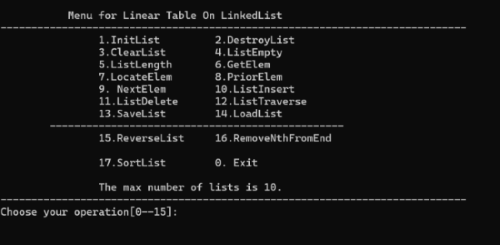
\includegraphics[width=1\linewidth]{Data_Structure/images/1.0.png}
\vspace{-0.2cm}


\newpage
\subsection{系统测试}
程序开发及实现环境:Win11 下使用 VScode+gcc 进行编译和调试,开发语言为 C 语言。

\quad 表\ref{table3.1}为正常样例测试的输入,预期结果与实际输出。
\begin{table}[p]
	\centering
	\caption{正常样例测试}
	\label{table3.1}
	\scalebox{0.7}{
		\begin{tabular}{|l|l|l|l|}
			\hline
			函数       & 输入                                                      & 实际输出                                                       &预期结果        \\ \hline
			初始化表      & 1                                                          & \begin{minipage}[b]{0.3\columnwidth} \centering \raisebox{-.5\height}{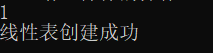
\includegraphics[width=\linewidth]{images/1.4.1.png}} \end{minipage}              &线性表创建成功    \\ \hline
			销毁表      & 2                                                          & \begin{minipage}[b]{0.3\columnwidth} \centering \raisebox{-.5\height}{
\includegraphics[width=\linewidth]{images/1.4.2.png}} \end{minipage}              &线性表销毁成功    \\ \hline
			销毁表      & 2                                                          & \begin{minipage}[b]{0.3\columnwidth} \centering \raisebox{-.5\height}{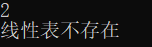
\includegraphics[width=\linewidth]{images/1.4.3.png}} \end{minipage}              &线性表不存在    \\ \hline
			初始化表      & 1                                                          & \begin{minipage}[b]{0.3\columnwidth} \centering \raisebox{-.5\height}{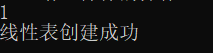
\includegraphics[width=\linewidth]{images/1.4.4.png}} \end{minipage}              &线性表创建成功    \\ \hline
			线性表判空      & 4                                                          & \begin{minipage}[b]{0.3\columnwidth} \centering \raisebox{-.5\height}{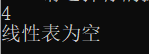
\includegraphics[width=\linewidth]{images/1.4.5.png}} \end{minipage}              &线性表为空    \\ \hline
			插入元素     & 10 1 1                                                          & \begin{minipage}[b]{0.3\columnwidth} \centering \raisebox{-.5\height}{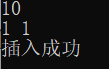
\includegraphics[width=\linewidth]{images/1.4.6.png}} \end{minipage}              &插入成功    \\ \hline
			插入元素      & 10 2 5                                                          & \begin{minipage}[b]{0.3\columnwidth} \centering \raisebox{-.5\height}{
\includegraphics[width=\linewidth]{images/1.4.7.png}} \end{minipage}              &插入成功    \\ \hline
			插入元素     & 10 3 7                                                          & \begin{minipage}[b]{0.3\columnwidth} \centering \raisebox{-.5\height}{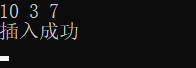
\includegraphics[width=\linewidth]{images/1.4.8.png}} \end{minipage}              &插入成功   \\ \hline
			求表长      & 5                                                          & \begin{minipage}[b]{0.3\columnwidth} \centering \raisebox{-.5\height}{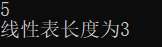
\includegraphics[width=\linewidth]{images/1.4.9.png}} \end{minipage}              &线性表长度为 3   \\ \hline
			获取元素      & 6 2                                                          & \begin{minipage}[b]{0.3\columnwidth} \centering \raisebox{-.5\height}{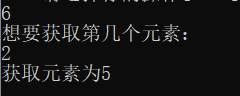
\includegraphics[width=\linewidth]{images/1.4.10.png}} \end{minipage}              &获取元素为 5    \\ \hline
			查找元素      & 7 7                                                          & \begin{minipage}[b]{0.3\columnwidth} \centering \raisebox{-.5\height}{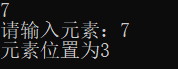
\includegraphics[width=\linewidth]{images/1.4.11.png}} \end{minipage}              &元素位置为 3    \\ \hline
			查找前驱      & 8 5                                                          & \begin{minipage}[b]{0.3\columnwidth} \centering \raisebox{-.5\height}{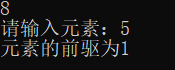
\includegraphics[width=\linewidth]{images/1.4.12.png}} \end{minipage}              &元素的前驱为 1  \\ \hline
			查找后继      & 9 5                                                          & \begin{minipage}[b]{0.3\columnwidth} \centering \raisebox{-.5\height}{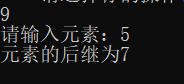
\includegraphics[width=\linewidth]{images/1.4.13.png}} \end{minipage}              &元素的后继为 7    \\ \hline
			遍历      & 12                                                          & \begin{minipage}[b]{0.3\columnwidth} \centering \raisebox{-.5\height}{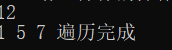
\includegraphics[width=\linewidth]{images/1.4.14.png}} \end{minipage}              &1 5 7 遍历完成    \\ \hline
			删除元素      & 11 2                                                          & \begin{minipage}[b]{0.3\columnwidth} \centering \raisebox{-.5\height}{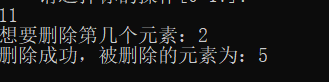
\includegraphics[width=\linewidth]{images/1.4.15.png}} \end{minipage}              &删除元素5   \\ \hline
			保存文件      & 13 123                                                          & \begin{minipage}[b]{0.3\columnwidth} \centering \raisebox{-.5\height}{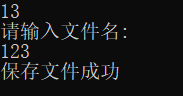
\includegraphics[width=\linewidth]{images/1.4.16.png}} \end{minipage}              &保存文件成功     \\ \hline
			销毁表      & 2                                                          & \begin{minipage}[b]{0.3\columnwidth} \centering \raisebox{-.5\height}{
\includegraphics[width=\linewidth]{images/1.4.17.png}} \end{minipage}              &线性表销毁成功    \\ \hline
			读取文件      & 17 F”:/shiyan                                                         & \begin{minipage}[b]{0.3\columnwidth} \centering \raisebox{-.5\height}{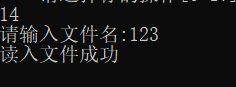
\includegraphics[width=\linewidth]{images/1.4.18.png}} \end{minipage}              &读入文件成功    \\ \hline
			遍历链表      & 12                                                          & \begin{minipage}[b]{0.3\columnwidth} \centering \raisebox{-.5\height}{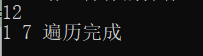
\includegraphics[width=\linewidth]{images/1.4.19.png}} \end{minipage}              &1 7 遍历完成    \\ \hline
		\end{tabular}
	}
\end{table}


\quad 表\ref{table3.2}为异常样例的输入,实际输出和对输出结果的分析\\
\begin{table}[b]
	\centering
	\caption{异常样例测试}
	\label{table3.2}
	\scalebox{0.7}{
		\begin{tabular}{|l|l|l|l|}
			\hline
			异常样例    & 输入            & 实际输出                                                                 & 结果分析       \\ \hline
			销毁表      & 2                                                          & \begin{minipage}[b]{0.3\columnwidth} \centering \raisebox{-.5\height}{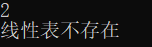
\includegraphics[width=\linewidth]{images/1.4.20.png}} \end{minipage}              &线性表不存在    \\ \hline
			清空表      & 3                                                          & \begin{minipage}[b]{0.3\columnwidth} \centering \raisebox{-.5\height}{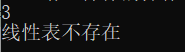
\includegraphics[width=\linewidth]{images/1.4.21.png}} \end{minipage}              &线性表不存在    \\ \hline
			获取元素 & 6                                                             & \begin{minipage}[b]{0.3\columnwidth} \centering 
				\raisebox{-.5\height}{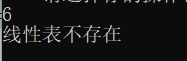
\includegraphics[width=\linewidth]{images/1.4.22.png}} \end{minipage}              &线性表不存在   \\ \hline
			查找后继 & 9 3                                                           & \begin{minipage}[b]{0.3\columnwidth} \centering \raisebox{-.5\height}{
\includegraphics[width=\linewidth]{images/1.4.23.png}} \end{minipage}                     &元素3没有后继元素  \\ \hline          
			插入元素 & 10 5 5                                                        & \begin{minipage}[b]{0.3\columnwidth} \centering \raisebox{-.5\height}{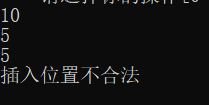
\includegraphics[width=\linewidth]{images/1.4.24.png}} \end{minipage}                     &插入元素的位置不合法  \\ \hline    
			读取文件 & 17                                                            & \begin{minipage}[b]{0.3\columnwidth} \centering \raisebox{-.5\height}{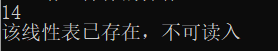
\includegraphics[width=\linewidth]{images/1.4.25.png}} \end{minipage}                    &线性表已存在   \\ \hline
		\end{tabular}
	}
\end{table}
\quad 通过异常用例可以看出,演示系统对表不存在时对除创建表以外的操作和对查找表中没有的元素的前驱、后继或对无后继、无前驱的元素要求获取后继、前驱的操作,以及在表存在时要求读取文件的操作的判定能力,可见演示系统能够识别异常样例。
\clearpage

\subsection{实验小结}

本次实验让我对基于链式存储结构的线性表有更进一步的了解。\par
演示系统的搭建,让我体会到了如何搭建一个可以调用不同模块的系统。\par
在编写插入和删除乃至翻转链表的函数时,如何有条理地更改指针的指向是一大难点。通过这次实验,我深刻的感受到了赋值顺序对程序的巨大影响。\par
总的来说,本次数据结构实验提高了我的编程能力,让我对系统的整体设计有了更深的认识。

\newpage
\section{基于邻接表的图实现}

\subsection{问题描述}
\noindent 实验要求:
\begin{enumerate}
	\item 实现对图的基本操作;
	\item 选择性实践对图的进阶操作;
	\item 设计演示系统。
\end{enumerate}
通过实验达到:
\begin{enumerate}
	\item 加深对图的概念、基本运算的理解;	
	\item 熟练掌握图的逻辑结构与物理结构的关系;
	\item 以邻接表作为物理结构,熟练掌握图基本运算的实现。
\end{enumerate}

\subsection{系统设计}
\subsubsection{演示系统菜单的组织架构}
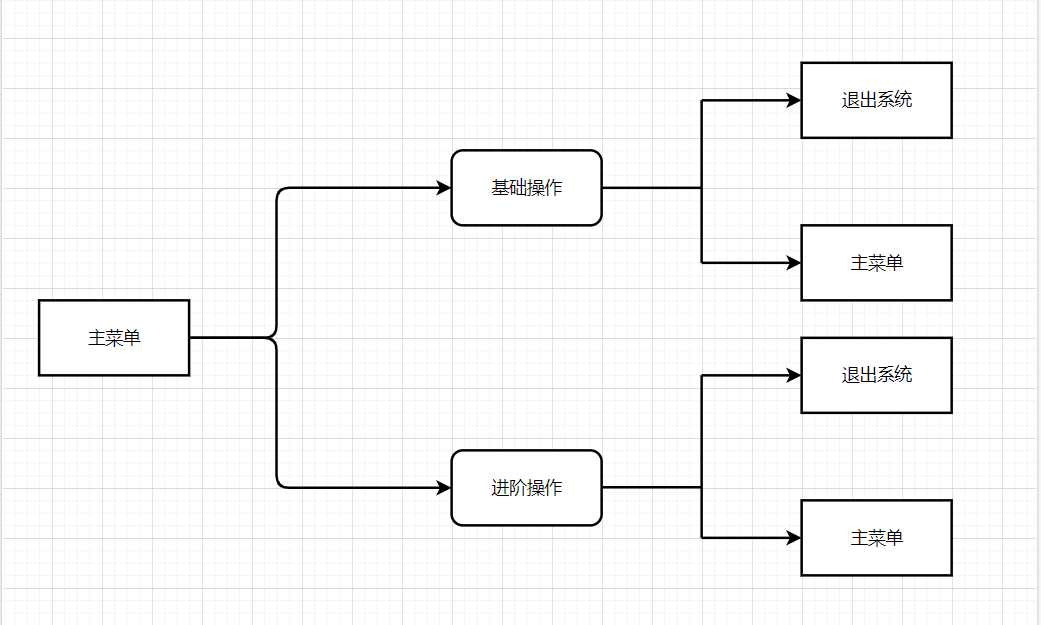
\includegraphics[width=1\linewidth]{Data_Structure/images/2.3.png}
\vspace{-0.2cm}
\newpage
\quad 演示系统分为基本操作和进阶操作两部分,以一个菜单为主界面,以序号1至12表示创建,销毁,清空,插入,删除,遍历等基本操作,以序号13至17表示保存为文件,求最短通路,求距某顶点距离小于d的顶点,对顶点进行修改等进阶操作,以序号0表示退出演示系统,根据序号调用函数执行操作。
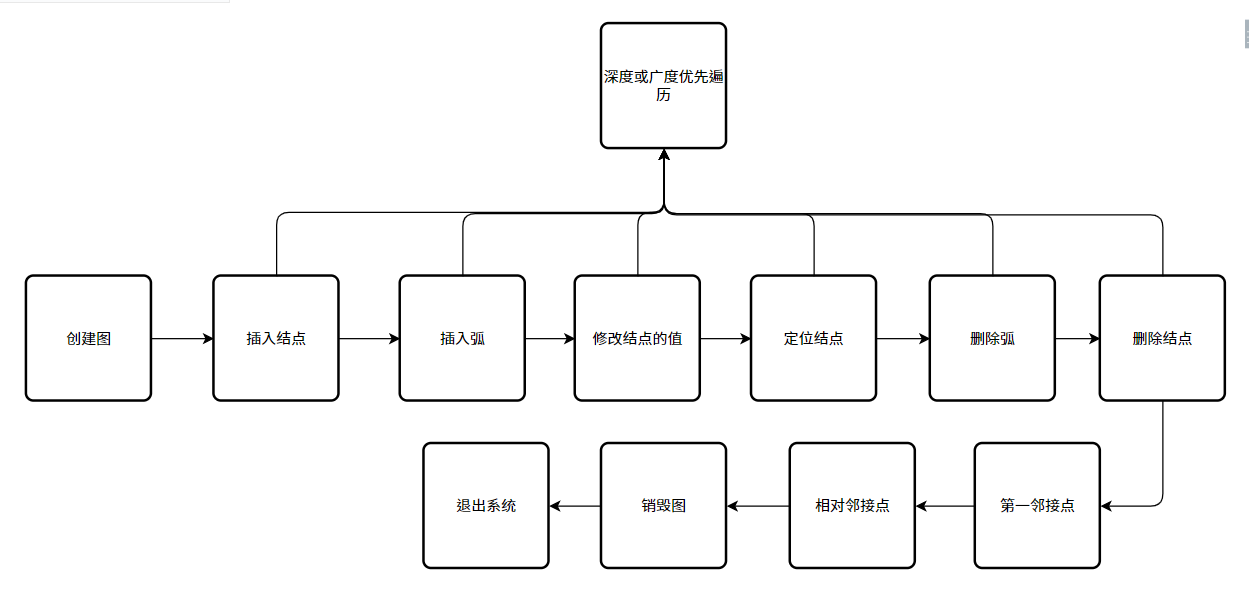
\includegraphics[width=1\linewidth]{Data_Structure/images/2.4.png}
\vspace{-0.2cm}
\subsubsection{ADT数据结构设计}
\noindent 对图数据类型的定义如下:\par
\begin{lstlisting}[language=C] 
typedef int status;
typedef int KeyType; 
typedef enum {DG,DN,UDG,UDN} GraphKind;

typedef struct {
    KeyType  key;
    char others[20];
} VertexType;//顶点类型定义

typedef struct ArcNode {//表结点类型定义
   	int adjvex;//顶点位置编号 
    struct ArcNode  *nextarc;//下一个表结点指针
} ArcNode;

typedef struct VNode{//头结点及其数组类型定义
   	VertexType data;//顶点信息
    ArcNode *firstarc;//指向第一条弧
} VNode,AdjList[MAX_VERTEX_NUM];

typedef  struct {//邻接表的类型定义
    AdjList vertices;//头结点数组
    int vexnum,arcnum;//顶点数、弧数
    GraphKind  kind;//图的类型
} ALGraph;	
\end{lstlisting}
对一些常量的定义如下:
\begin{lstlisting}[language=C] 
#define TRUE 1
#define FALSE 0
#define OK 1
#define ERROR 0
#define INFEASIBLE -1
#define OVERFLOW -2
#define MAX_VERTEX_NUM 20
\end{lstlisting}

\subsubsection{创建图}
输入:图G(未知状态),顶点集 V[] , 边集 VR[]

输出:函数执行状态

算法的思想描述:定义 vexnum=0,arcnum=0,分别记录顶点和边的数目。
如若当前顶点序列的关键字不为-1 执行 while 循环:如果当前关键字未出现
则更新标记数组并继续,否则返回 ERROR,在邻接表添加新顶点,令表头
结点为 NULL,更新顶点数,检查是否超过最大数目MAXVERTEXNUM ,超过则返回 ERROR。
循环结束如果vexnum=0,即没有顶点,则返回ERROR,否则令G.vexnum=vexnum。
当当前关系序列不为 (-1,-1) 时执行 while 循环:用 for 循环遍历邻接表,查
找关系序列相应顶点

\begin{lstlisting}[language=C] 
status CreateCraph(ALGraph &G,VertexType V[],KeyType VR[][2])
/*根据V和VR构造图T并返回OK,如果V和VR不正确,返回ERROR
如果有相同的关键字,返回ERROR。此题允许通过增加其它函数辅助实现本关任务*/
{
    int i=0,j=0;
    while(V[i].key!=-1)
    {
        for(int k=0;k<i;k++)
            if(V[i].key==V[k].key) 
                return ERROR;

        if(i>=MAX_VERTEX_NUM) 
            return ERROR;
        G.vertices[i].data=V[i];//赋值
		G.vertices[i].firstarc=NULL;
		i++;
    }
    if(i==0) 
        return ERROR;
    G.vexnum=i;//顶点数

    while(VR[j][0]!=-1)
    {
        int a=Locate(G,VR[j][0]),b=Locate(G,VR[j][1]);
        if(!(a>=0&&b>=0)) 
            return ERROR;
        ArcNode *q=(ArcNode*)malloc(sizeof(ArcNode)) ;
        q->adjvex=b;
        q->nextarc=G.vertices[a].firstarc;//头插法
        G.vertices[a].firstarc=q;
        q=(ArcNode*)malloc(sizeof(ArcNode)) ;
        q->adjvex=a;
        q->nextarc=G.vertices[b].firstarc;//头插法
        G.vertices[b].firstarc=q;
        j++;
    }
    G.arcnum=j;
    return OK;
}
\end{lstlisting}

时间复杂度:O(n)

空间复杂度:O(n)


\subsubsection{销毁图}

输入:图G

输出:函数执行状态

算法的思想描述:遍历所有弧结点
\begin{lstlisting}{language=C}
status DestroyGraph(ALGraph &G)
/*销毁无向图G,删除G的全部顶点和边*/
{
    ArcNode *p=NULL,*q=NULL;
    for(int k=0;k<G.vexnum;k++)
    {
        if(G.vertices[k].firstarc!=NULL)//释放边
        {
            p=G.vertices[k].firstarc;
            while(p!=NULL)
            {
                q=p->nextarc;//释放
                free(p);
                p=q;
            }
            G.vertices[k].firstarc=NULL;
        }
    }
    G.arcnum=0;
	G.vexnum=0;
    return OK;
}
\end{lstlisting}
算法处理步骤:
\begin{enumerate}
	\renewcommand{\labelenumi}{\theenumi)}
	\item 用两个临时变量分别记录首节点与下一结点。
	\item 删除首个顶点然后两个结点开始移动,遍历完一个顶点的所有邻接点。
	\item 重复直至所有结点都遍历过。
	\item 删除成功,返回 OK。
\end{enumerate}

时间复杂度:O(n)

空间复杂度:O(1)

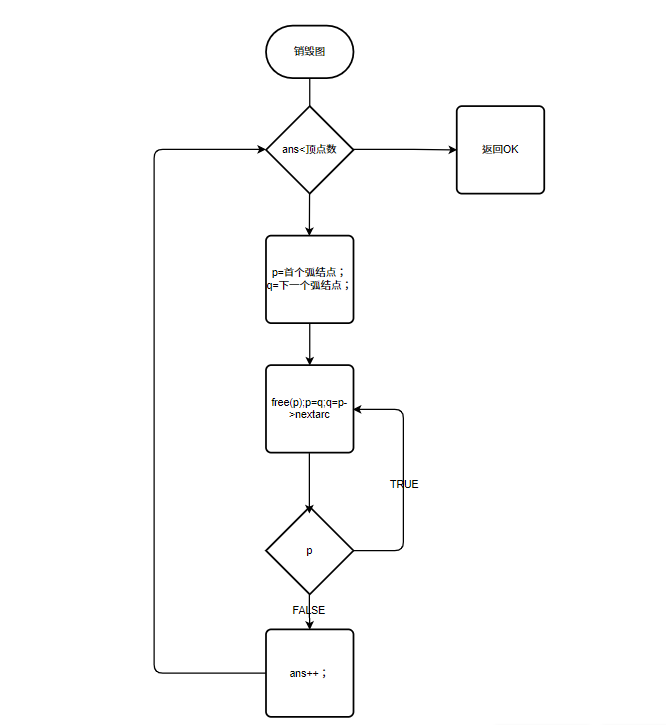
\includegraphics[width=1\linewidth]{Data_Structure/images/2.3.2.png}
\vspace{-0.2cm}
\subsubsection{定位顶点}
输入:图G, 要查找顶点的关键字

输出:要查找顶点的位序

算法的思想描述:用 for 循环遍历邻接表,如果当前顶点关键字与所找关键字相等,则返回当前顶点序号。如果没找到,返回-1。
\begin{lstlisting}[language=C] 	
int LocateVex(ALGraph G,KeyType u)
//根据u在图G中查找顶点,查找成功返回位序,否则返回-1;
{
    int i=0;
    for(i;i<G.vexnum;i++)
        if(G.vertices[i].data.key==u) //找到
            return i;
    
    return -1;
}
\end{lstlisting}

时间复杂度:O(n)

空间复杂度:O(1)
\subsubsection{修改顶点}
输入:图G,要修改结点的关键字,以及要修改成的值value

输出:函数执行状态

算法的思想描述:寻找赋值顶点并赋值
\begin{lstlisting}{language=C}
status PutVex(ALGraph &G,KeyType u,VertexType value)
//根据u在图G中查找顶点,查找成功将该顶点值修改成value,返回OK;
//如果查找失败或关键字不唯一,返回ERROR
{
    int i=0;
    for(;i<G.vexnum;i++)
        if(G.vertices[i].data.key==u) 
        {
            for(int k=0;k<G.vexnum;k++)
                // if(G.vertices[k].data.key==value.key) //找到
                //     return ERROR;
            
            G.vertices[i].data=value;  
            return OK;
        }
    
    return ERROR;  
}
\end{lstlisting}
算法处理步骤:
\begin{enumerate}
	\renewcommand{\labelenumi}{\theenumi)}
	\item 定位需要赋值的顶点的位置。
	\item 将该顶点的关键字和值域重新赋值。
	\item 修改成功,返回 OK。
\end{enumerate}

时间复杂度:O(n)

空间复杂度:O(1)

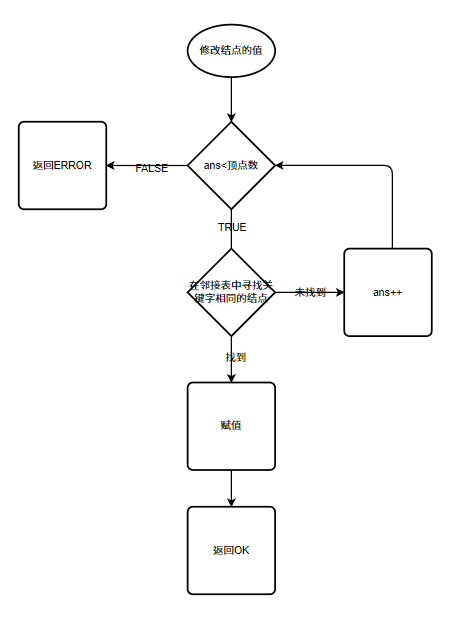
\includegraphics[width=1\linewidth]{Data_Structure/images/2.3.3.png}
\vspace{-0.2cm}
\subsubsection{第一邻接点}

输入:图G,要查找邻接点的顶点的关键字

输出:第一邻接点的位序

算法思想描述:调用定位函数查找关键字为u的结点。如果 i == G.vexnum || G.vertices[i].firstarc == NULL,即没找到该点或该点无
邻接点,则返回-1。否则返回 G.vertices[i].firstarc->adjvex。
\begin{lstlisting}{language=C}
int FirstAdjVex(ALGraph G,KeyType u)
//根据u在图G中查找顶点,查找成功返回顶点u的第一邻接顶点位序,否则返回-1;
{
    int i=0;
    for(;i<G.vexnum;i++)
        if(G.vertices[i].data.key==u&&G.vertices[i].firstarc) 
            return G.vertices[i].firstarc->adjvex;//找到
    return -1;
}

\end{lstlisting}
算法处理步骤:
\begin{enumerate}
	\renewcommand{\labelenumi}{\theenumi)}
	\item 定位关键字为 v 的顶点的位置.
	\item 若下一个弧结点不为空则返回它否则返回-1。
\end{enumerate}

时间复杂度:O(n)

空间复杂度:O(1)

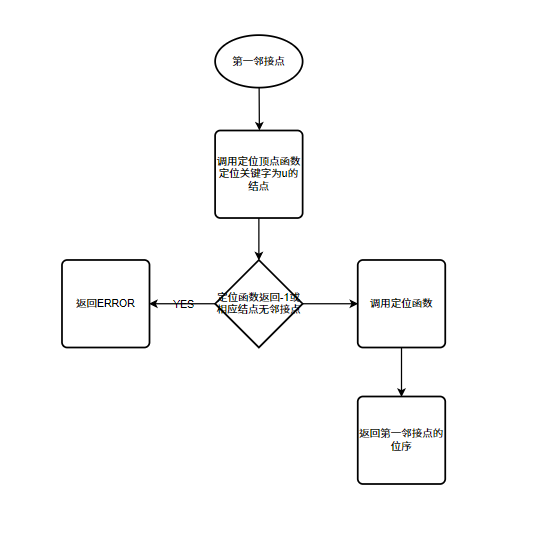
\includegraphics[width=1\linewidth]{Data_Structure/images/2.3.4.png}
\vspace{-0.2cm}
\subsubsection{下一邻接点}
输入:图G,要查找邻接点的顶点的关键字

输出:下一邻接点的位序

算法的思想描述:调用定位函数查找关键字为u的结点。如果 i==G.vexnum,返回ERROR。用 while 循环遍历该顶点的所有邻接点,找到另个一顶点,用 p 指向该邻接点。如果 p == NULL || p->nextarc == NULL,即 v 与 w 不相邻,或 v 相对 w无下一邻接点,返回-1。否则返回 return p->nextarc->adjvex。

\begin{lstlisting}[language=C] 
int NextAdjVex(ALGraph G,KeyType v,KeyType w)
//v对应G的一个顶点,w对应v的邻接顶点;操作结果是返回v的(相对于w)下一个邻接顶点的位序;如果w是最后一个邻接顶点,或v、w对应顶点不存在,则返回-1。
{
    int i=LocateVex(G,v);
    int j=LocateVex(G,w);
    while(i!=-1&&j!=-1)
    {
        if(G.vertices[i].firstarc==NULL) 
            return -1;
        else
        {
            ArcNode *p=G.vertices[i].firstarc;//找到
            while(p->adjvex!=j&&p)
                p=p->nextarc;
            
            if(p->nextarc)
                return p->nextarc->adjvex;
            else 
                return -1;
        }
    }
    return -1;
}
\end{lstlisting}

时间复杂度:O(n)

空间复杂度:O(1)
\subsubsection{插入顶点}
输入:图G,要插入顶点的关键字

输出:函数执行状态

算法的思想描述:如果 G.vexnum == MAXVERTEXNUM,返回 ERROR。如若不然使用 LocateVex 查找要插入结点的关键字。如果要插入顶点的关键字已出现,则返回 ERROR。否则插入新顶点,更新顶点数,返回 OK。
\begin{lstlisting}[language=C] 
status InsertVex(ALGraph *G,VertexType v)
//在图G中插入顶点v,成功返回OK,否则返回ERROR
{
    if(LocateVex(*G,v.key)>=0) 
        return ERROR;
    if((*G).vexnum==MAX_VERTEX_NUM) 
        return ERROR;
    (*G).vertices[(*G).vexnum].data=v;//赋值
    (*G).vertices[(*G).vexnum].firstarc=NULL;
    (*G).vexnum++;
    return OK;
}
\end{lstlisting}

时间复杂度:O(n)

空间复杂度:O(1)

\subsubsection{删除顶点}

输入:图G,要删除的顶点的关键字

输出:函数的执行状态.

算法思想的描述:寻找所要删除的顶点,记录它所连接的所有弧结点 ,在其他顶点中将所有的弧结点删除

\begin{lstlisting}[language=C] 
status DeleteVex(ALGraph &G,KeyType v)
//在图G中删除关键字v对应的顶点以及相关的弧,成功返回OK,否则返回ERROR
{
    int i=LocateVex(G,v),j=-1;
    if(i==-1) 
        return ERROR;
    if(G.vexnum==1 || G.vexnum==0)
        return ERROR;
    ArcNode *p=G.vertices[i].firstarc;
    ArcNode *q=NULL;
    ArcNode *temp=NULL;
    while(p)
    {  
        j=p->adjvex;
        q=G.vertices[j].firstarc;
        if(q->adjvex==i)
        {
            temp=q;
            G.vertices[j].firstarc=q->nextarc;
            free(temp); 
        }
        else
        {
            while(q->nextarc->adjvex!=i)
                q=q->nextarc;
            
            temp=q->nextarc;
            q->nextarc=temp->nextarc;//删除
            free(temp);
        }
        temp=p->nextarc;
        free(p);
        p=temp;
        G.arcnum--;
    }
    for(int k=i;k<G.vexnum;k++)
        G.vertices[k]=G.vertices[k+1];//删除    
    
    G.vexnum--;
    for(int k=0;k<G.vexnum;k++)
	{
		p=G.vertices[k].firstarc;
		while(p!=NULL)
		{
			if(p->adjvex>i)
			    p->adjvex--;
			p=p->nextarc;
		}
	}
    return OK;
}
\end{lstlisting}

时间复杂度:O(n*n)

空间复杂度:O(1)

\subsubsection{插入弧}
输入:图 G,和顶点关键字类型相同的给定值v,w

输出:函数执行状态

算法的思想描述:查找 v,w 的关键字,如果其中任意一个未找到,则返回 ERROR,否则分别在这两个关键字后的链表中添加相应弧,返回 OK。	
\begin{lstlisting}{language=C}
status InsertArc(ALGraph &G,KeyType v,KeyType w)
//在图G中增加弧<v,w>,成功返回OK,否则返回ERROR
{
    int i=LocateVex(G,v);
    int j=LocateVex(G,w);
    if(i==-1||j==-1) 
        return ERROR;
    if(LocateArc(G,v,w)!=ERROR) 
        return ERROR;
    ArcNode *p=(ArcNode*)malloc(sizeof(ArcNode));//插入<v,w>
    p->adjvex=j;
    p->nextarc=G.vertices[i].firstarc;
    G.vertices[i].firstarc=p;
    p=(ArcNode*)malloc(sizeof(ArcNode));
    p->adjvex=i;
    p->nextarc=G.vertices[j].firstarc;
    G.vertices[j].firstarc=p;
    G.arcnum++;
    return OK;
}
\end{lstlisting}
算法处理步骤:
\begin{enumerate}
	\renewcommand{\labelenumi}{\theenumi)}
	\item 寻找所要插入的结点 v,w
	\item 在 v 和 w 中分别用首插法
	\item 总弧数加 1 。
\end{enumerate}

时间复杂度:O(n)

空间复杂度:O(1)


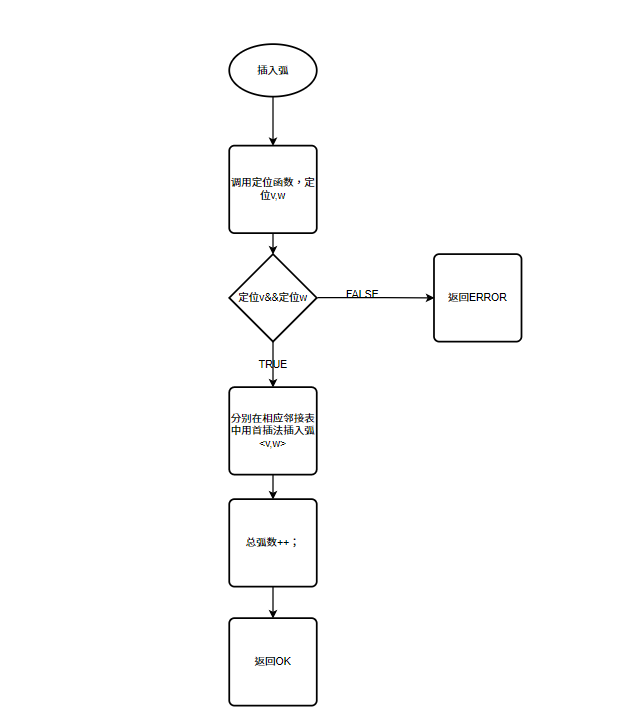
\includegraphics[width=1\linewidth]{Data_Structure/images/2.3.5.png}
\vspace{-0.2cm}
\subsubsection{删除弧}

输入:图 G,和顶点关键字类型相同的给定值v,w

输出:函数的执行状态。

算法的思想描述:调用函数查找 v,w 的关键字,如果其中任意一个未找到,则返回 ERROR,否则分别在这两个关键字后的链表中寻找并删除对应结点的弧,返回 OK。	
\begin{lstlisting}{language=C}
status DeleteArc(ALGraph &G,KeyType v,KeyType w)
//在图G中删除弧<v,w>,成功返回OK,否则返回ERROR
{
    if(LocateArc(G,v,w)==ERROR) 
        return ERROR;
    int i=LocateVex(G,v);
    int j=LocateVex(G,w);//删除<v,w>
    ArcNode *p=G.vertices[i].firstarc;//删除<v,w>
    ArcNode *temp=NULL;
    if(p->adjvex==j)
    {
        temp=p;
        G.vertices[i].firstarc=p->nextarc;//删除<v,w>
        free(temp);
    }
    else 
    {
        while(p->nextarc->adjvex!=j)
            p=p->nextarc;
        
        temp=p->nextarc;
        p->nextarc=p->nextarc->nextarc;//删除<v,w>
        free(temp);
    }
    p=G.vertices[j].firstarc;//删除<v,w>的对称弧<w,v>
    temp=NULL;//删除<v,w>的对称弧<w,v>
    if(p->adjvex==i)
    {
        temp=p;
        G.vertices[j].firstarc=p->nextarc;
        free(temp);
    }
    else 
    {
        while(p->nextarc->adjvex!=i)
            p=p->nextarc;

        temp=p->nextarc;
        p->nextarc=p->nextarc->nextarc;
        free(temp);
    }
    G.arcnum--;
    return OK;
}
\end{lstlisting}
算法处理步骤:
\begin{enumerate}
	\renewcommand{\labelenumi}{\theenumi)}
	\item 寻找所要删除的弧的信息。
	\item 分别在 v 中删除 w 和在 w 中删除 v。
	\item 若删除成功则返回 OK。
\end{enumerate}

时间复杂度:O(n)

空间复杂度:O(1)


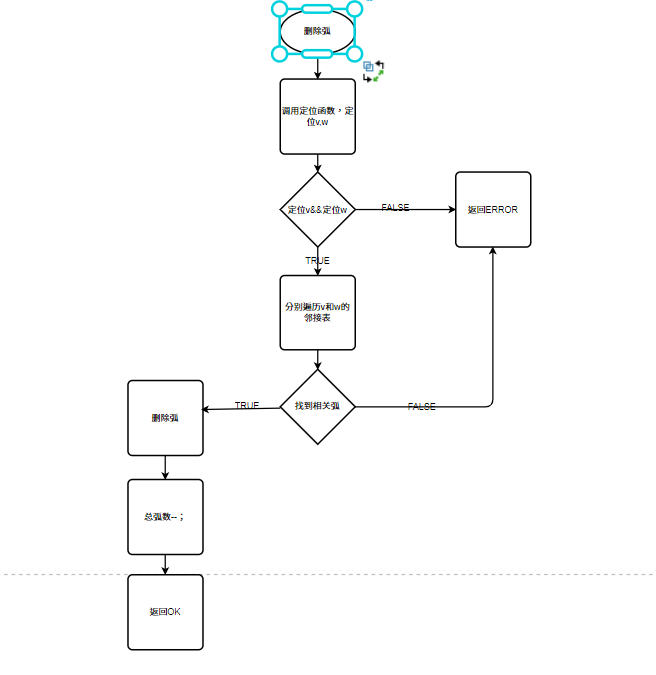
\includegraphics[width=1\linewidth]{Data_Structure/images/2.3.6.png}
\vspace{-0.2cm}
\subsubsection{深度优先遍历}
输入: 图 G

输出:函数执行状态

算法的思想描述:定义标记数组用于标记顶点是否已访问;递归地从第一个顶点开始访问其余顶点,每次访问时更新标记数组,以确保每个节点只被访问一次;返回 OK。
\begin{lstlisting}{language=C}
void dfs(ALGraph &G,KeyType v,void(*visit)(VertexType))
{
	visited[v]=TRUE;
	int x=LocateVex(G,v);
	visit(G.vertices[x].data);//访问顶点v
	for(int w=FirstAdjVex(G,v);w>=0;w=NextAdjVex(G,v,G.vertices[w].data.key)) 
		if(!visited[G.vertices[w].data.key])
            dfs(G,G.vertices[w].data.key,visit);//递归调用
}


status DFSTraverse(ALGraph &G,void(*visit)(VertexType))
{
	int i;
	for(i=0;i<G.vexnum;i++)
	    visited[G.vertices[i].data.key]=FALSE;//标记数组记录关键字 

	for(i=0;i<G.vexnum;i++)
		if(!visited[G.vertices[i].data.key])//若未访问
			dfs(G,G.vertices[i].data.key,visit);
	
	return OK;
} 
\end{lstlisting}
算法处理步骤:
\begin{enumerate}
	\renewcommand{\labelenumi}{\theenumi)}
	\item  构造一个对一个顶点所有邻接结点的递归函数fps
	\item  依次读取每个顶点并用标记数组记录已读取的顶点
	\item  用 visit 函数将深度遍历的结点信息逐个打印。
\end{enumerate}

时间复杂度:O(n)

空间复杂度:O(1)

\subsubsection{广度优先遍历}
输入:图G

输出:函数的执行状态

算法思想描述:利用队列这一数据结构, 保存每一次广搜的所有弧结点并将他们在下一次广搜时访问所有未被读取的首节点。
\begin{lstlisting}[language=C] 
status InitQueue(Linkqueue &Q)
{
	Q.front=Q.rear=(QNode *)malloc(sizeof(QNode));
	if(!Q.front)
        return ERROR;
	Q.front->next=NULL;//头结点指针域置空
	return OK;
} 


status QueueEmpty(Linkqueue Q)
{
	if(Q.front==Q.rear)
        return TRUE;//队列为空
	else 
        return FALSE;
}


status enQueue(Linkqueue &Q,VertexType value)
{
	Queue p=(Queue)malloc(sizeof(QNode));
	if(!p)
        return ERROR;
	p->data=value;
	p->next=NULL;//新结点指针域置空
	Q.rear->next=p;
	Q.rear=p;
	return OK;
}


status deQueue(Linkqueue &Q,VertexType &value)
{
	if(Q.front==Q.rear)
        return ERROR;
	Queue p=Q.front->next;
	value=p->data;
	Q.front->next=p->next;
	if(Q.rear==p)
	    Q.rear=Q.front;
	free(p);
	return OK;
}


status BFSTraverse(ALGraph &G,void (*visit)(VertexType))
//对图G进行广度优先搜索遍历,依次对图中的每一个顶点使用函数visit访问一次,且仅访问一次
{
	int i=0,j;
	VertexType value;
	Linkqueue Q;
	InitQueue(Q);
	for(i=0;i<G.vexnum;i++)
		visited[G.vertices[i].data.key]=FALSE;  //标记数组记录关键字
	
for(i=0;i<G.vexnum;i++)
    if(!visited[G.vertices[i].data.key])
    {
        visited[G.vertices[i].data.key]=TRUE;//标记已访问
        visit(G.vertices[i].data);
        enQueue(Q,G.vertices[i].data);
        while(!QueueEmpty(Q))
        {
            deQueue(Q,value);
            for(int w=FirstAdjVex(G,value.key);w>=0;w=NextAdjVex(G,value.key,G.vertices[w].data.key))
                if(!visited[G.vertices[w].data.key])//如果未访问过
                {
                    visited[G.vertices[w].data.key]=TRUE;//标记已访问
                    visit(G.vertices[w].data);
                    enQueue(Q,G.vertices[w].data);
                }
            
        }
    }
	
	return OK;
}
\end{lstlisting}

时间的复杂度:O(n).

空间的复杂度:O(n).
\newpage 

\subsection{系统实现}

\subsubsection{程序开发环境与语言}
程序开发及实现环境:Win11 下使用 VScode+gcc 进行编译和调试,开发语言为 C 语言。
\subsubsection{代码的组织结构}
演示系统以一个菜单作为交互界面,用户通过输入命令对应的编号来调用相应的函数来实现创建图,销毁图,清空图,插入顶点,删除顶点,遍历等基本操作,以及保存为文件,求最短通路,求距某顶点距离小于d的顶点,对顶点进行修改等进阶操作。


程序主函数为一个switch结构,根据输入的数字,执行不同的语句,进而调用不同的函数,宏定义函数返回值ERROR为0,INFEASIBLE为-1,OVERFLOW为-2,OK为1.
交互界面如下图



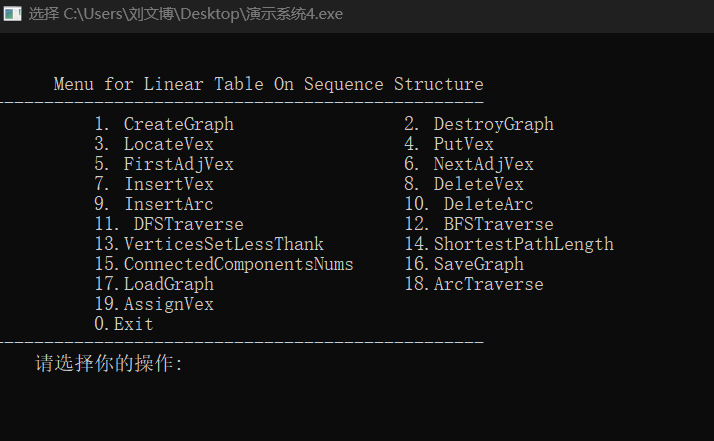
\includegraphics[width=1\linewidth]{Data_Structure/images/2.3.1.png}
\vspace{-0.2cm}
\clearpage

\subsection{系统测试}
程序开发及实现环境:Win11 下使用 VScode+gcc 进行编译和调试,开发语言为 C 语言。\par

表\ref{table3.3}为正常样例测试的输入,预期结果与实际输出\par
\begin{table}[htbp]
	\centering
	\caption{正常样例测试}
	\label{table3.3}
	\scalebox{0.7}{
		\begin{tabular}{|l|l|l|l|}
			\hline
			函数       & 输入                                                      & 实际输出                                                       &预期结果        \\ \hline
			创建图      & 5..5 6 5 7 6 7 7 8 -1 -1                                                         & \begin{minipage}[b]{0.3\columnwidth} \centering \raisebox{-.5\height}{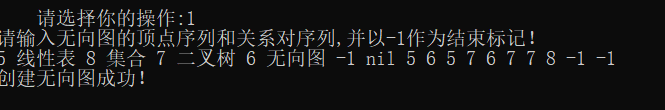
\includegraphics[width=\linewidth]{images/2.4.1.png}} \end{minipage}              &创建无向图成功    \\ \hline
			定位顶点      & 8                                                          & \begin{minipage}[b]{0.3\columnwidth} \centering \raisebox{-.5\height}{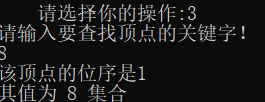
\includegraphics[width=\linewidth]{images/2.4.2.png}} \end{minipage}              &返回关键字为8的顶点的位序1    \\ \hline
			修改顶点      & 6 9 有向图                                                         & \begin{minipage}[b]{0.3\columnwidth} \centering \raisebox{-.5\height}{
\includegraphics[width=\linewidth]{images/2.4.4.png}} \end{minipage}              &修改成功    \\ \hline
			查找第一邻接点     & 7                                                          & \begin{minipage}[b]{0.3\columnwidth} \centering \raisebox{-.5\height}{
\includegraphics[width=\linewidth]{images/2.4.6.png}} \end{minipage}              &该顶点的第一邻接顶点的位序为1  其值为8 集合   \\ \hline
			查找下一邻接点     & 7 8                                                          & \begin{minipage}[b]{0.3\columnwidth} \centering \raisebox{-.5\height}{
\includegraphics[width=\linewidth]{images/2.4.9.png}} \end{minipage}              &顶点7的邻接顶点相对于8的下一邻接顶点的位序是3
			其值为 6 无向图    \\ \hline
			深度优先遍历     & 11                                                        & \begin{minipage}[b]{0.3\columnwidth} \centering \raisebox{-.5\height}{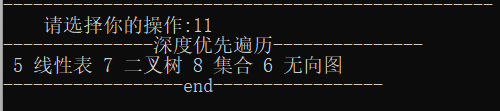
\includegraphics[width=\linewidth]{images/2.4.10.png}} \end{minipage}              & 5 线性表 7 二叉树 8 集合 6 无向图   \\ \hline
			广度优先遍历      & 12                                                          & \begin{minipage}[b]{0.3\columnwidth} \centering \raisebox{-.5\height}{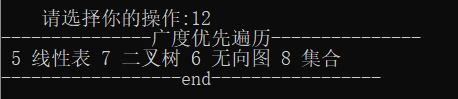
\includegraphics[width=\linewidth]{images/2.4.11.png}} \end{minipage}              & 5 线性表 7 二叉树 6 无向图 8 集合   \\ \hline
			销毁图      & 2                                                          & \begin{minipage}[b]{0.3\columnwidth} \centering \raisebox{-.5\height}{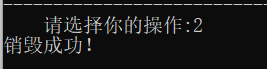
\includegraphics[width=\linewidth]{images/2.4.12.png}} \end{minipage}              &销毁成功    \\ \hline
		\end{tabular}
	}
\end{table}

表\ref{table3.4}为异常样例的输入,实际输出和对输出结果的分析\par

\begin{table}[htbp]
	\centering
	\caption{异常样例测试}
	\label{table3.4}
	\scalebox{0.7}{
		\begin{tabular}{|l|l|l|l|}
			\hline
			异常样例    & 输入            & 实际输出                                                                 & 结果分析       \\ \hline
			创建图      & 5 (略) 5 6 5 7 6 7 7 8 -1 -1                                                         & \begin{minipage}[b]{0.3\columnwidth} \centering \raisebox{-.5\height}{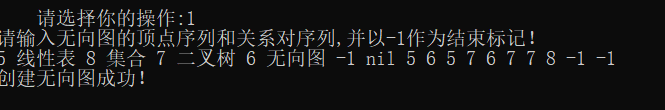
\includegraphics[width=\linewidth]{images/2.4.1.png}} \end{minipage}              &创建无向图成功    \\ \hline
			定位顶点      & 10                                                          & \begin{minipage}[b]{0.3\columnwidth} \centering \raisebox{-.5\height}{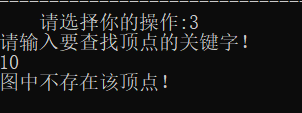
\includegraphics[width=\linewidth]{images/2.4.3.png}} \end{minipage}              &找不到关键字为10的顶点    \\ \hline
			修改顶点      & 6 5 有向图                                                        & \begin{minipage}[b]{0.3\columnwidth} \centering \raisebox{-.5\height}{
\includegraphics[width=\linewidth]{images/2.4.5.png}} \end{minipage}              &关键字为5的结点已存在   \\ \hline
			查找第一邻接点 & 10                                                           & \begin{minipage}[b]{0.3\columnwidth} \centering \raisebox{-.5\height}{
\includegraphics[width=\linewidth]{images/2.4.8.png}} \end{minipage}                     &找不到关键字为10的顶点  \\ \hline  
			销毁图 & 2                                                           & \begin{minipage}[b]{0.3\columnwidth} \centering \raisebox{-.5\height}{\includegraphics[width=\linewidth]{images/2.4.12.png}} \end{minipage}                     &销毁成功  \\ \hline    
			销毁图 & 2                                                           & \begin{minipage}[b]{0.3\columnwidth} \centering \raisebox{-.5\height}{\includegraphics[width=\linewidth]{images/2.4.13.png}} \end{minipage}                     &图还未创建,无法销毁  \\ \hline         
		\end{tabular}
	}
\end{table}

通过异常用例可以看出,演示系统对要求插入与已有顶点关键字相同的顶点,和定位不包含在图中的顶点以及销毁还未创建的图等操作的判定能力,可见演示系统能够识别异常样例。




\subsection{实验小结}
本次实验让我对基于邻接表的图实现的了解更进了一步。\\
演示系统的搭建,让我体会到了主函数和子函数的关系,以及如何搭建一个可以调用不同模块的系统。\par
在编写插入和删除弧的函数时,如何有效地根据关键字找到相应结点是使程序变得简洁的一大关键,在编写插入与删除弧的函数时,如果能够在之前定义定位顶点的函数并调用,将极大地省去冗杂的代码,这次实验让我对函数的工具性,模块性有了直观的感受。\par
总的来说,本次数据结构实验提高了我的编程能力,让我对系统整体设计有了更深的认识。\par
相比之前几次的实验,图的系统实现更为复杂,进阶操作的实现需要了解一些经典的算法,本次实验让我有了较大的进步。
\newpage

\section{课程的收获和建议}
\subsection{基于链式存储结构的线性表实现}
通过对基于链式存储结构的线性表实现的演示系统练习,我基本掌握了线性表的基本操作,能够根据需要调用不同的模块来灵活地使用线性表这一数据结构。\par
\subsection{基于邻接表的图实现}
数据结构这门课里最复杂的数据结构就是图,通过对基于邻接表的图实现的实验学习,我对数据结构的认识更加深入。\par





\section{附录A 基于顺序存储结构线性表实现的源程序}

\noindent

\begin{lstlisting}
/*SequenceList.cpp*/

#include"SequenceListFunc.h"

// main function
int main(void)
{
    SqList L; 
    L.elem=NULL; // Initialize the Sequence List
    int op=1;   
    int flag=0;

    while(op)
    {
        system("cls");	// Clear the screen

        // Menu
        printf("\n\n");
        printf("  Menu for Linear Table On Sequence Structure \n");
        printf("------------------------------\n");
        printf("    1. InitList       7. LocateElem\n");
        printf("    2. DestroyList    8. PriorElem\n");
        printf("    3. ClearList      9. NextElem \n");
        printf("    4. ListEmpty      10. ListInsert\n");
        printf("    5. ListLength     11. ListDelete\n");
        printf("    6. GetElem        12. ListTraverse\n");
         printf("    13.MaxSubArray    14.SubArrayNum\n");
        printf("    15.SortList       16.SaveList\n");
        printf("    17.LoadList\n");
        
        printf("    0. Exit\n");
        printf("---------------------------------\n");
        printf("Choose your operation[0~17]:\n");
        printf("Press Enter to continue after a certain operation...\n");
        

        // input the operation number
        scanf("%d",&op);


        // Switch the operation
        switch(op)
        {
            case 1:// InitList
            {
                if(InitList(L)==OK) 
                    printf("Success!\n");
                else 
                    printf("Failed!\n");

                getchar();// pause
                getchar();
                break;
            }

            case 2:// DestroyList
            {
                if(DestroyList(L)==OK)  
                    printf("Success!\n");
                else 
                    printf("Failed!\n");   

                getchar();// pause
                getchar();
                break;
            }

            case 3:// ClearList
            {
                if(ClearList(L)==OK)    
                    printf("Success!\n"); 
                else 
                    printf("Failed!\n");

                getchar();// pause
                getchar();
                break;
            }

            case 4:// ListEmpty
            {
                if(ListEmpty(L)==TRUE)   
                    printf("The Sequence List is empty!\n");
                else if(ListEmpty(L)==FALSE) 
                    printf("The Sequence List is not empty!\n");
                else 
                    printf("Failed!\n");

                getchar();// pause
                getchar();
                break;
            }

            case 5:// ListLength
            {
                if(ListLength(L)!=INFEASIBLE)
                {
                    int Length=0;
                    Length=ListLength(L);
                    printf("Success!");
                    printf("\n THe length of the Sequence List is %d .\n",Length);
                }
                else 
                    printf("Failed!\n");

                getchar();// pause
                getchar();
                break;
            }

            case 6:// GetElem
            {
                int i=0; 
                ElemType e=0;

                printf("Which element(->position) do you want to get?\n");
                scanf("%d",&i);

                if(GetElem(L,i,e)==ERROR)
                    printf("The value of i is illegal!\n");
                else if(GetElem(L,i,e)==INFEASIBLE) 
                    printf("Failed to get the element!\n");
                else if(GetElem(L,i,e)==OK) 
                {
                    printf("Success!\n");
                    printf("The element is %d .\n",e);
                }     

                getchar();// pause
                getchar();
                break;
            }

            case 7:// LocateElem
            {   
                int i=0;
                ElemType e=0;

                printf("Which element do you want to locate?\n");
                scanf("%d",&e);

                i=LocateElem(L,e);

                if(i==INFEASIBLE)
                    printf("The Sequence List is not exist!\n");
                if(i==0)
                    printf("The element is not exist.\n");
                if(i!=INFEASIBLE&&i!=0)
                    printf("The element is in the No.%d position.\n",i);

                getchar();// pause
                getchar();
                break;
            }

            case 8:// PriorElem
            {
                ElemType e=0;
                printf("Which elementdo you wanna get the prior element?\n");
                scanf("%d",&e);
                ElemType pre_e=0;

                if(PriorElem(L,e,pre_e)==ERROR)
                    printf("The element has no prior element!\n");
                if(PriorElem(L,e,pre_e)==INFEASIBLE)
                    printf("The Sequence List is not exist!\n");
                if(PriorElem(L,e,pre_e)==OK)
                {
                    printf("Success!\n");
                    printf("The prior element is %d .\n",pre_e);
                }  

                getchar();// pause
                getchar();
                break;
            }

            case 9:// NextElem
            {
                ElemType e=0;
                printf("Which element(->value) do you want to get the next element?\n");
                scanf("%d",&e);
                ElemType next_e=0;
                if(NextElem(L,e,next_e)==ERROR)
                    printf("The element has no next element!\n");
                if(NextElem(L,e,next_e)==INFEASIBLE)
                    printf("The Sequence List is not exist!\n");
                if(NextElem(L,e,next_e)==OK)
                {
                    printf("Success!\n");
                    printf("The next element is %d .\n",next_e);
                }   

                getchar();// pause
                getchar();
                break;
            }

            case 10:// ListInsert
            {   
                int i;
                ElemType e;
                printf("format: [serial number] [element]\n");
                scanf("%d%d", &i, &e);
                if(ListInsert(L, i, e)==OK) 
                    printf("Success!\n");
                else if(ListInsert(L, i, e)==INFEASIBLE) 
                    printf("Sequence is empty! Initialize first!\n");
                else 
                    printf("Insertion failed! Check your input!\n");

                getchar();// pause
                getchar();
                break;
            }

            case 11:// ListDelete
            {
                int i=0,j=0;
                ElemType e=0;
                printf("Which element(->serial number) do you want to delete?\n");
                scanf("%d",&i);
                j=ListDelete(L,i,e);
                if(j==ERROR)
                    printf("The position is illegal!\n");
                if(j==INFEASIBLE)
                    printf("The Sequence List is not exist!\n");
                if(j==OK)
                {
                    printf("Success!\n");
                    printf("The deleted element is %d .\n",e);
                }    

                getchar();// pause
                getchar();
                break;
            }

            case 12:// ListTraverse
            {
                if(!ListTraverse(L)) 
                    printf("The Sequence List is not exist!\n");

                getchar();// pause
                getchar();
                break;
            }

            case 13:// MaxSubArray
            {
                MaxSubArray(L);
                printf("The maximum sum of the subarray is %d .\n",ans);

                getchar();// pause
                getchar();
                break;
            }

            case 14:// SubArrayNum
            {
                int k=0;
                printf("Please input the sum of the subarray.\n");
                scanf("%d",&k); 
                SubArrayNum(L,k);
                printf("The number of the subarray whose sum is %d is %d .\n",k,ans);

                getchar();// pause
                getchar();
                break;
            }

            case 15:// SortList
            {
                printf("The Sequence List is being sorted.\n\n");
                SortList(L);

                getchar();// pause
                getchar();
                break;
            } 

            case 16:// SaveList
            {
                char FileName[100];
                printf("Please input the file name.\n");
                scanf("%s",&FileName); 
                if(SaveList(L,FileName))
                    printf("successfully!\n");
                else 
                    printf("Failed!\n");

                getchar();// pause
                getchar();
                break;
            }

            case 17:// LoadList
            {
                if(!L.elem)
                {
                    char FileName[100];
                    printf("Please input the file name.\n");
                    scanf("%s",&FileName); 
                    if(LoadList(L,FileName))
                        printf("The Sequence List has been loaded successfully!\n");
                    else 
                        printf("Failed!\n");

                    getchar();// pause
                    getchar();
                    break;
                }
                else
                {
                    printf("The Sequence List had existed!\n");

                    getchar();// pause
                    getchar();
                    break;
                }
            }

            case 0:// Exit
                break;
        }
    }
    printf("Bye!\n");
    return 0;
}
\end{lstlisting}
\newpage
\begin{lstlisting}
//SequenceListFunc.h

#include <stdio.h>
#include <malloc.h>
#include <stdlib.h>


#define TRUE 1
#define FALSE 0
#define OK 1
#define ERROR 0
#define INFEASIBLE -1
#define OVERFLOW -2
#define LIST_INIT_SIZE 100
#define LISTINCREMENT  10

typedef int status; 
typedef int ElemType; 

typedef struct{ 
	ElemType * elem;
	int length;
	int listsize;
}SqList;//type of Sequence List


// Function declaration
status InitList(SqList& L);
status DestroyList(SqList& L);
status ClearList(SqList&L);
status ListEmpty(SqList L);
int ListLength(SqList L);
status GetElem(SqList L,int i,ElemType& e);
status LocateElem(SqList L,ElemType e); 
status PriorElem(SqList L,ElemType cur,ElemType &pre_e);
status NextElem(SqList L,ElemType cur,ElemType &next_e);
status ListInsert(SqList &L,int i,ElemType e);
status ListDelete(SqList&L,int i,ElemType& e);
status ListTraverse(SqList L); 
status MaxSubArray(SqList L);
status SubArrayNum(SqList L,int k);
status SortList(SqList &L);
status SaveList(SqList L,char Filename[]);
status LoadList(SqList &L,char Filename[]);

int ans=0,sum=0;

// function definition

    status InitList(SqList& L)
    // 线性表L不存在,构造一个空的线性表,
    //返回OK,否则返回INFEASIBLE。
    {
        if(L.elem==NULL)
        {
            L.elem=(ElemType*)malloc(LIST_INIT_SIZE*sizeof(ElemType));
            L.length=0;
            L.listsize=LIST_INIT_SIZE;
            return OK;
        }
        else
            return INFEASIBLE;
    }


    status DestroyList(SqList &L)
    // 如果线性表L存在,销毁线性表L,释放数据元素的空间,
    //返回OK,否则返回INFEASIBLE。
    {
        if(L.elem!=NULL)
        {
            free(L.elem);
            L.elem=NULL;
            L.length=0;
            L.listsize=0;
            return OK;
        }
        else 
            return INFEASIBLE;
    }


    status ClearList(SqList& L)
    // 如果线性表L存在,删除线性表L中的所有元素,
    //返回OK,否则返回INFEASIBLE。
    {
        if(L.elem!=NULL)
        {
            int length = L.length;
            int i;

            for (i = 0; i < length; i++)
                L.elem[i] = 0;

            L.length = 0;
            return OK;
        }
        else
            return INFEASIBLE;
    }



    status ListEmpty(SqList L)
    // 如果线性表L存在,判断线性表L是否为空,空就返回TRUE,
    //否则返回FALSE;如果线性表L不存在,返回INFEASIBLE。
    {
        if(L.elem==NULL)
            return INFEASIBLE;
        else
            if(L.length==0)
                return TRUE;
            else
                return FALSE;
    }


    status ListLength(SqList L)
    // 如果线性表L存在,返回线性表L的长度,否则返回INFEASIBLE。
    {
        if(L.elem!=NULL)
            return L.length;
        else
            return INFEASIBLE;
    }


    status GetElem(SqList L,int i,ElemType &e)
    // 如果线性表L存在,获取线性表L的第i个元素,保存在e中,返回OK;
    //如果i不合法,返回ERROR;如果线性表L不存在,返回INFEASIBLE。
    {
        if (L.elem==NULL)
            return INFEASIBLE;
        else if(L.elem!=NULL&&(i<1||i>L.length))
            return ERROR;
        e=L.elem[i-1];
        return OK;
    }


    int LocateElem(SqList L,ElemType e)
    // 如果线性表L存在,查找元素e在线性表L中的位置序号并返回该序号;
    //如果e不存在,返回0;当线性表L不存在时,返回INFEASIBLE(即-1)。
    {
        if(L.elem!=NULL)
        {
            int i=1;
            while(L.elem[i-1]!=e&&(i-1)<=L.length-1)
                i++;

            if(i>=1&&i<=L.length)
                return i;
            else
                return 0;
        }
        else 
            return INFEASIBLE;
    }


    status PriorElem(SqList L,ElemType e,ElemType &pre)
    // 如果线性表L存在,获取线性表L中元素e的前驱,保存在pre中,返回OK;
    //如果没有前驱,返回ERROR;如果线性表L不存在,返回INFEASIBLE。
    {
        if(L.elem!=NULL)
        {
            int i=0;
            if(L.elem[i]==e) 
                return ERROR;
            else 
            {
                i=1;
                while(i<L.length)
                {
                    if(L.elem[i]==e) 
                    {
                        pre=L.elem[i-1];
                        return OK;
                    }
                    else 
                        i++;
                }
                return ERROR;
            }
        }
        else 
            return INFEASIBLE;
    }


    status NextElem(SqList L,ElemType e,ElemType &next)
    // 如果线性表L存在,获取线性表L元素e的后继,保存在next中,返回OK;
    //如果没有后继,返回ERROR;如果线性表L不存在,返回INFEASIBLE。
    {
        if(L.elem!=NULL)
        {
            int i=L.length-1;
            if(L.elem[i]==e)
                return ERROR;
            else
            {
                i=i-1;
                while(i>=0)
                {
                    if(L.elem[i]==e)
                    {
                        next=L.elem[i+1];
                        return OK;
                    }
                    i--;
                }
                if(i<0)
                    return ERROR;
            }
        }
        else
            return INFEASIBLE;
        return ERROR;
    }


    status ListInsert(SqList &L,int i,ElemType e)
    // 如果线性表L存在,将元素e插入到线性表L的第i个元素之前,返回OK;
    //当插入位置不正确时,返回ERROR;如果线性表L不存在,返回INFEASIBLE。
    {
        if(L.elem==NULL)
            return INFEASIBLE;
        if(L.length>=L.listsize)
        {
            ElemType *newbase=(ElemType*)realloc(L.elem,(L.listsize+LISTINCREMENT)*sizeof(ElemType));
            L.elem=newbase;
            L.listsize+=LISTINCREMENT;
        }
        if(L.elem!=NULL)
        {
            if(L.length==0)
            {
                L.elem[0]=e;
                L.length++;
                return OK;
            }
            if(i>=1&&i<=L.length+1)
            {
                for(int j=L.length;j>=i;j--)
                    L.elem[j]=L.elem[j-1];

                L.elem[i-1]=e;
                L.length++;
                return OK;
            }
        }
        return ERROR;
    }


    status ListDelete(SqList &L,int i,ElemType &e)
    // 如果线性表L存在,删除线性表L的第i个元素,并保存在e中,返回OK;
    //当删除位置不正确时,返回ERROR;如果线性表L不存在,返回INFEASIBLE。
    {
        if(L.elem)
        {
            if((i<1)||(i>L.length))
                return ERROR;

            int *p,*q;

            p=&(L.elem[i-1]);
            e=*p;
            q=L.elem+L.length-1;

            for(++p;p<=q;++p)
                *(p-1)=*p;

            L.length--;
            return OK;
        }
        else 
            return INFEASIBLE;
    }


    status ListTraverse(SqList L)
    // 如果线性表L存在,依次显示线性表中的元素,每个元素间空一格,
    //返回OK;如果线性表L不存在,返回INFEASIBLE。
    {
        if(L.elem==NULL)
            return INFEASIBLE;
        if(L.length>=L.listsize)
        {
            ElemType *newbase=(ElemType*)realloc(L.elem,(L.listsize+LISTINCREMENT)*sizeof(ElemType));
            L.elem=newbase;
            L.listsize+=LISTINCREMENT;
        }
        if(L.elem)
        {
            if(L.length)
            {
                printf("======= Elements in Sequence List =======\n\n");
                for(int i=0;i<L.length;i++)
                {
                    if(i != L.length-1)
                        printf("%d ",L.elem[i]);
                    else
                        printf("%d\n\n",L.elem[i]);
                }
                printf("==================================\n");
            }
            return OK;
        }
        return L.length;
    }


    status MaxSubArray(SqList L)
    // 初始条件是线性表L已存在且非空,请找出一个具有最大和的连续子数组
    //(子数组最少包含一个元素),操作结果是其最大和;
    {
        sum=0;
        ans=0;
        if(!L.elem) 
            return ERROR;
        for(int i=0;i<L.length;i++)
        {
            sum+=L.elem[i];
            if(ans<sum)
                ans=sum;
        }
        return OK;
    }


    status SubArrayNum(SqList L,int k)
    // 初始条件是线性表L已存在且非空,
    //请找出一个具有和为k的连续子数组的个数,操作结果是其个数;
    {
        ans=0;
        if(!L.elem)     
            return ERROR;
        for(int i=0;i<L.length;i++)
        {
            sum=0;
            for(int j=i;j<L.length;j++)
            {
                sum+=L.elem[j];
                if(sum==k) 
                    ans++;
            }
        }
        return OK;
    }


    status SortList(SqList &L)
    // 如果线性表L存在,将线性表L中的元素按从小到大的顺序排列,返回OK;
    //如果线性表L不存在,返回INFEASIBLE。
    {
        if(!L.elem) 
            return ERROR;
        int temp=0;
        
        for(int i=0;i<L.length-1;i++)
            for(int j=0;j<L.length-1-i;j++)
                if(L.elem[j]>L.elem[j+1])
                {
                    temp=L.elem[j];
                    L.elem[j]=L.elem[j+1];
                    L.elem[j+1]=temp; 
                }
        ListTraverse(L);
        return OK;
    }


    status  SaveList(SqList L,char FileName[])
    // 如果线性表L存在,将线性表L的的元素写到FileName文件中,
    //返回OK,否则返回INFEASIBLE。
    {
        if(L.elem==NULL)
            return INFEASIBLE;
        else
        {
            FILE *fp=fopen(FileName,"w");
            if(!fp)
                return ERROR;

            fprintf(fp,"%d\n",L.length);

            for(int i=0;i<L.length;i++)
                fprintf(fp,"%d ",L.elem[i]);
            
            fclose(fp);
            return OK;
        }
    }


    status  LoadList(SqList &L,char FileName[])
    // 如果线性表L不存在,将FileName文件中的数据读入到线性表L中,
    //返回OK,否则返回INFEASIBLE。
    {

        if(L.elem!=NULL)
            return INFEASIBLE;
        else
        {
            L.elem=(ElemType*)malloc(LIST_INIT_SIZE*sizeof(ElemType));
            L.length=0;
            L.listsize=LIST_INIT_SIZE;
            FILE *fp=fopen(FileName,"r");
            if(!fp)
                return ERROR;
            fscanf(fp,"%d",&L.length);
            for(int i=0;i<L.length;i++)
                fscanf(fp,"%d",&L.elem[i]);
            
            fclose(fp);
            return OK;
        }
    }
\end{lstlisting}
\newpage


\section{附录B 基于链式存储结构线性表实现的源程序}
\begin{lstlisting}
//LinkedList.cpp

#include "LinkedListFunc.h"

//main function
int main()
{
char filename[40];
int op=1;
    int i,flag=0,i_num=0;
    LinkList L[MAX_NUM];


    for (i = 0; i<MAX_NUM; i++)
    	L[i]=NULL;

ElemType e, cur_e, pre_e, next_e;


    while(op)
{
system("cls");

printf("\n\n");
printf("  	   Menu for Linear Table On LinkedList \n");
printf("     		1.InitList         2.DestroyList\n");
printf("     		3.ClearList        4.ListEmpty\n");
printf("     		5.ListLength       6.GetElem \n");
printf("    		7.LocateElem       8.PriorElem \n");
printf("     		9. NextElem        10.ListInsert\n");
printf("     		11.ListDelete      12.ListTraverse\n");
printf("     		13.SaveList        14.LoadList\n");
printf("     		15.ReverseList     16.RemoveNthFromEnd\n\n");
printf("     		17.SortList        0. Exit\n\n");
printf("		The max number of lists is %d.\n", MAX_NUM);

printf("Choose your operation[0--15]:\n");
scanf("%d",&op);


switch(op)
{
case 1://InitList
if(InitList(&L[i_num])==OK)
{
printf("Input the filename to save the list:\n");
scanf("%s", filename);
printf("Success!\n");
}
else 
printf("Failed!\n");

getchar();
getchar();
break;

case 2://DestroyList
if(L[i_num] == NULL)
{
printf("The list doesn't exist!\n");

getchar();
getchar();
break;
}
if(DestroyList(&L[i_num])==OK)
printf("Success!\n");
else 
printf("Failed!\n");

getchar();
getchar();
break;

case 3://ClearList
if(L[i_num] == NULL)
{
printf("The list doesn't exist!\n");

getchar();
getchar();
break;
}
if(ClearList(&L[i_num])==OK)
printf("Success!\n");
else 
printf("Failed!\n");

getchar();
getchar();
break;

case 4://ListEmpty
if(L[i_num] == NULL)
{
printf("The list doesn't exist!\n");

getchar();
getchar();
break;
}
if(ListEmpty(L[i_num])==TRUE)
printf("The file is empty!\n");

else 
printf("The file is not empty!\n");

getchar();
getchar();
break;

case 5://ListLength
if(L[i_num] == NULL)
{
printf("The list doesn't exist!\n");

getchar();
getchar();
break;
}
printf("The length of the list is %d\n",ListLength(L[i_num]));

getchar();
getchar();
break;

case 6://GetElem
if(L[i_num] == NULL)
{
printf("The list doesn't exist!\n");

getchar();
getchar();
break;
}
printf("Input the position of the element you wanna get:\n");
scanf("%d",&i);
if(GetElem(L[i_num],i,&e)==OK)
printf("The element of the position %d is %d\n",i,e);
else  
printf("The position is invalid!\n");

getchar();
getchar();
break;

case 7://LocateElem
if(L[i_num] == NULL)
{
printf("The list doesn't exist!\n");

getchar();
getchar();
break;
}
printf("Input the element you wanna locate:\n");

scanf("%d",&e);

if(i=LocateElem(L[i_num],e,compare))
printf("The element %d is in the position %d\n",e,i);
else  
printf("The element doesn't exist!\n");

getchar();
getchar();
break;

case 8://PriorElem
if(L[i_num] == NULL)
{
printf("The list doesn't exist!\n");

getchar();
getchar();
break;
}
printf("Input the element you wanna get its prior element:\n");

scanf("%d",&cur_e);

PriorElem(L[i_num],cur_e,&pre_e);

if(PriorElem(L[i_num],cur_e,&pre_e)==OK)
printf("The prior element of %d is %d\n",cur_e,pre_e);
else if(PriorElem(L[i_num],cur_e,&pre_e)==OVERFLOW)
printf("The element doesn't exist!\n");
else 
printf("The element doesn't have a prior element!\n");

getchar();
getchar();
break;


case 9://NextElem
if(L[i_num] == NULL)
{
printf("The list doesn't exist!\n");

getchar();
getchar();
break;
}
printf("Input the element you wanna get its next element:\n");

scanf("%d",&cur_e);

if(NextElem(L[i_num],cur_e,&next_e)==OK)
printf("The next element of %d is %d\n",cur_e,next_e);
else if(NextElem(L[i_num],cur_e,&pre_e)==ERROR)
printf("The element doesn't exist!\n");
else
printf("The element doesn't have a next element!\n");

getchar();
getchar();
break;

case 10://ListInsert
if(L[i_num] == NULL)
{
printf("The list doesn't exist!\n");

getchar();
getchar();
break;
}
printf("Input the element and its position :\n");
printf("format:[position] [element]\n");

scanf("%d %d",&i,&e);

if(ListInsert(&L[i_num],i,e)==OK)
printf("Success!\n");
else
printf("Failed!\n");

getchar();
getchar();
break;

case 11://ListDelete
if(L[i_num] == NULL)
{
printf("The list doesn't exist!\n");

getchar();
getchar();
break;
}
printf("Input the position of the element you wanna delete:\n");
scanf("%d",&i);
if(ListDelete(&L[i_num],i,&e)==OK)
printf("Success!\n");
else
printf("Failed!\n");

getchar();
getchar();
break;

case 12://ListTrabverse
if(L[i_num] == NULL)
{
printf("The list doesn't exist!\n");

getchar();
getchar();
break;
}
if(ListTrabverse(L[i_num])==0) 
printf("The list is empty!\n");

getchar();
getchar();
break;

case 13://SaveList
if(L[i_num] == NULL)
{
printf("The list doesn't exist!\n");

getchar();
getchar();
break;
}
if(SaveList(L[i_num], filename)==OK)
printf("file named %s has been saved!\n",filename);

getchar();
getchar();
break;

case 14://LoadList
InitList(&L[i_num]);

printf("Input the filename you wanna load:\n");

scanf("%s", filename);

if(LoadList(&L[i_num], filename)==OK)
printf("file named %s has been loaded!\n",filename);
getchar();
getchar();
break;

case 15://ReverseList
flag=ReverseList(&L[i_num]);
if(flag== INFEASIBLE) 
printf("The list doesn't exist!\n");
else if(flag == ERROR) 
printf("The list is empty!\n");
else
printf("Success!\n");

getchar(); 
getchar();
break;


case 16://RemoveNthFromEnd
printf("Input the position of the element you wanna delete:\n");
scanf("%d",&i);
flag=RemoveNthFromEnd(L[i_num],i,e);
if(flag== INFEASIBLE) 
printf("The list doesn't exist!\n");
else if(flag == ERROR) 
printf("The list is empty!\n");
else
printf("Success!\n");

getchar(); 
getchar();
break;


case 17://SortList
flag=SortList(L[i_num]);
if(flag== INFEASIBLE) 
printf("The list doesn't exist!\n");
else if(flag == ERROR) 
printf("The list is empty!\n");
else
printf("Success!\n");

getchar(); 
getchar();
break;

case 0://Exit
break;
}
}
printf("Bye!\n");
}
\end{lstlisting}
\newpage
\begin{lstlisting}
//LinkedListFunc.h

 #include <stdio.h>
 #include <malloc.h>
 #include <stdlib.h>
 
 
 #define TRUE 1
 #define FALSE 0
 #define OK 1
 #define ERROR 0
 #define INFEASIBLE -1
 #define OVERFLOW -2
 #define MAX_NUM 10
 #define LIST_INIT_SIZE 100
 #define LISTINCREMENT  10
 
 
typedef int status;
typedef int ElemType; //type of element
 
 
typedef struct LNode{
ElemType data;
struct LNode *next;
 }LNode, *LinkList;
 
 
FILE *fp;//file pointer
 
 
 //initiate the functions
status InitList(LinkList *L);
status DestroyList(LinkList *L);
status ClearList(LinkList *L);
status ListEmpty(LinkList L);
int ListLength(LinkList L);
status GetElem(LinkList L, int i, ElemType *e);
int LocateElem(LinkList L, ElemType e, status(*compare)(ElemType a, ElemType b));
status compare(ElemType a, ElemType b);
status PriorElem(LinkList L, ElemType cur_e, ElemType *pre_e);
status NextElem(LinkList L, ElemType cur_e, ElemType *next_e);
status ListInsert(LinkList *L, int i, ElemType e);
status ListDelete(LinkList *L, int i,ElemType *e);
status ListTrabverse(LinkList L);
status SaveList(LinkList L, char* filename);
status LoadList(LinkList *L, char *filename);
status ReverseList(LinkList *L);
 
status InitList(LinkList *L)
 //initiate a list
 {
 *L = (LinkList)malloc(sizeof(LNode));//malloc a node
if(*L == NULL)
 {
exit(OVERFLOW);//malloc failed
 }
 (*L)->data = 0;
 (*L)->next = NULL;//the list is empty
return OK;
 }
 
 
 
status DestroyList(LinkList *L)
 //destroy a list
 {
LinkList p, q;
p = *L;
while(p)
 {
q = p->next;
free(p);
p = q;
 }
 *L = NULL;
return OK;
 }
 
 
status ClearList(LinkList *L)
 //clear a list
 {
LinkList p, q;
p = (*L)->next;//point to the first node
while(p)
 {
q = p->next;
free(p);
p = q;
 }
 (*L)->next = NULL;
return OK;
 }
 
 
status ListEmpty(LinkList L)
 //judge if the list is empty
 {
if(L->next)
return FALSE;
else
return TRUE;
 }
 
 
int ListLength(LinkList L)
 //get the length of the list
 {
int i = 0;
LinkList p = L->next;
while(p)
 {
i++;
p = p->next;
 }
return i;
 }
 
 
 
status GetElem(LinkList L, int i, ElemType *e)
 //get the element of the No.i node
 {
int j = 1;
LinkList p;
p = L->next;
while(p && j < i)
 {
p = p->next;
 ++j;
 }
if(!p || j>i)
return ERROR;
 *e = p->data;
return OK;
 }
 
 
int LocateElem(LinkList L, ElemType e, status(*compare)(ElemType a, ElemType b))
 //get the position of the element
 {
int i = 0;
LinkList p = L->next;
while(p)
 {
i++;
if((*compare)(p->data, e))
return i;
p = p->next;
 }
return 0;
 }
 
status compare(ElemType a, ElemType b)
 {
if(a == b)
return TRUE;
else
return FALSE;
 }
 
 
 
status PriorElem(LinkList L, ElemType cur_e, ElemType *pre_e)
 //get the element before the cur_e
 {
LinkList p = L->next;
if(p->data==cur_e) 
return ERROR;
while(p->next != NULL && p->next->data != cur_e)
p = p->next;
 
if(p->next == NULL)
return OVERFLOW;
 
 *pre_e = p->data;
return OK;
 }
 
 
 
status NextElem(LinkList L, ElemType cur_e, ElemType *next_e)
 //get the element after the cur_e
 {
LinkList p = L->next;
while(p->next != NULL && p->data != cur_e)
p = p->next;
 
if(p->next == NULL && p->data != cur_e)	
return ERROR;
if(p->next == NULL && p->data == cur_e)	
return OVERFLOW;
 *next_e = p->next->data;	
return OK;
 }
 
 
 
status ListInsert(LinkList *L, int i, ElemType e)
 //insert a node before the No.i node
 {
int j = 1;
LinkList p, q;
p = *L;
while(p && j < i)
 {
p = p->next;
 ++j;
 }
if(!p || j > i)
return ERROR;
 
q = (LinkList)malloc(sizeof(LNode));
if(q == NULL)
exit(OVERFLOW);
 
q->data = e;
q->next = p->next;
p->next = q;
return OK;
 }
 
 
 
status ListDelete(LinkList *L, int i,ElemType *e)
 //delete the No.i node
 {
int j = 1;
LinkList p ,q;
p = *L;
while(p->next && j < i)
 {
p = p->next;
 ++j;
 }
if(!(p->next) || j>i)
return ERROR;
 
q = p->next;
p->next = q->next;
 *e = q->data;
free(q);
 
return OK;
 }
 
 
 
status ListTrabverse(LinkList L)
 //traverse the list
 {
    LinkList p = L;
     if(!p)
         return INFEASIBLE;
     else if (!p->next)
         return ERROR;
     else
     {
         while(p)
         {
             if(p->data!=0)
                 printf("%d ",p->data);	
             p = p->next;
         }
         return OK;
     }
 }
 
 
 
status SaveList(LinkList L, char* filename)
 //save the list to a file
 {
LinkList p = L->next;
int listsize=LIST_INIT_SIZE;	
if ((fp = fopen(filename, "w")) == NULL)
 {
printf("File open error!\n");
return ERROR;
 }
fprintf(fp, "%d ", ListLength(L));
fprintf(fp, "%d ", listsize);
while(p)
     {
fprintf(fp, "%d ", p->data);
p = p->next;
     }
fclose(fp);
return OK;
 }
 
 
 
status LoadList(LinkList *L, char *filename)
 //load the list from a file
 {
int i = 1,length = 0,listsize;
ElemType e;
if ((fp = fopen(filename, "r")) == NULL)
 {
printf("File open error!\n");
return ERROR;
 }
fscanf(fp, "%d ", &length);
fscanf(fp, "%d ", &listsize);
fscanf(fp, "%d ", &e);
while(i<=length)
     {
ListInsert(L,i,e);
fscanf(fp, "%d ", &e);
i++;
     }
fclose(fp);
return OK;
 }
 
 
status ReverseList(LinkList *L)
 //reverse the list
 {
     if(L)
     {
         LinkList prev=NULL;
LinkList cur=*L;
LinkList next=NULL;
while(cur)
 {
next=cur->next;
cur->next=prev;
prev=cur;
cur=next;
 }
 *L=prev;
return OK;
 }
     else  
return INFEASIBLE;
 }
 
 
status RemoveNthFromEnd(LinkList &L, int n, ElemType& e)
 //delete the nth node from the end of the list
 {
     if(!L) 
return INFEASIBLE;
     else
 {
int k,j; 
         if(L->next==NULL) 
return ERROR;
         k = ListLength(L);
         j = k - n + 1;
         ListDelete(&L, j, &e);
         return OK;
     }
 }
 
 
status SortList(LinkList L)
 // sort the list
 {
     LinkList p, q;
     if(!L) 
return INFEASIBLE;
     else
 {
         if(L->next==NULL) 
return ERROR;
         int n = ListLength(L);
         int i, j, temp;
         for(i = 0,p = L -> next; i < n-1; i++,p = p -> next)
             for(j = i + 1,q = p -> next; j < n; j++,q = q -> next)
                 if(p -> data > q -> data)
 {
                     temp = p -> data;
                     p -> data = q -> data;
                     q -> data = temp;
                 }
 
         return OK;
     }
 }
\end{lstlisting}
\newpage
\section{附录C 基于二叉链表二叉树实现的源程序}
\begin{lstlisting}
//BinaryTree.cpp
#include "BinaryTreeFunc.h"


int main()
{
int op=1,flag=0,i,lr;
KeyType key,key1,key2;

BiTree T=NULL;
BiTNode* t;
char FileName[30],TreeName[30];
T=NULL; 

while(op)
{
system("cls");

printf("\n\n");
printf("      Menu for Linear Table On Sequence Structure \n");
printf("    	  1. CreateBiTree           2. DestroyBiTree\n");
printf("    	  3. ClearBiTree            4. BiTreeEmpty\n");
printf("    	  5. BiTreeDepth            6. LocateNode\n");
printf("    	  7. Assign                 8. GetSibling\n");
printf("    	  9. InsertNode             10.DeleteNode\n");
printf("    	  11.PreOrderTraverse       12.InOrderTraverse\n");
printf("    	  13.PostOrderTraverse      14.LevelOrderTraverse\n");
printf("    	  15.MaxPathSum             16.LowestCommonAncestor\n");
printf("    	  17.InvertTree             18.SaveBiTree\n");
printf("    	  19.LoadBiTree             0. Exit\n");
printf("Choose your operation[0~19]:\n");


scanf("%d",&op);


switch(op)
{
case 1://CreateBiTree
if(T)  
printf("The tree has been existed!\n");
else
{
printf("Please input the definition of the tree with empty node:\n");
i=0;
do
{
scanf("%d%s",&definition[i].key,definition[i].others);//输入结点的值
} while (definition[i++].key!=-1);
flag=CreateBiTree(T,definition);//创建二叉树
if(flag==1)
printf("The tree has been created successfully!\n");
else if(flag==0)
printf("The tree has been created failed!\n");
}
getchar();
getchar();
break;


case 2://DestroyBiTree
flag=DestroyBiTree(&T);//销毁二叉树
if(flag==1)
printf("The tree has been destroyed successfully!\n");
else 
printf("The tree has been destroyed failed!\n");
getchar();
getchar();
break;


case 3://ClearBiTree
if(!T)
printf("The tree has not been created!\n");
else
{
flag=ClearBiTree(T);//清空二叉树
if(flag==OK)
printf("The tree has been cleared successfully!\n");
else 
printf("The tree has been cleared failed!\n");
}
getchar();
getchar();
break;


case 4://BiTreeEmpty
flag=BiTreeEmpty(T);
if(flag==1)
printf("The tree is empty!\n");
else if(flag==0)
printf("The tree is not empty!\n");
else 
printf("The tree has not been created!\n");

getchar();
printf("Press Enter to continue...");
getchar();
break;


case 5://BiTreeDepth
flag=BiTreeDepth(T);//求二叉树的深度
if(flag!=-1) 
printf("The depth of the tree is %d.\n",flag);
else 
printf("The tree has not been created!\n");
getchar();
getchar();
break;


case 6://LocateNode
if(!T)
printf("The tree has not been created!\n");
else
{
printf("Please input the key of the node:");
scanf("%d",&key);
t=LocateNode(T,key);
if(t)  
printf("The node is (%d,%s).\n",t->data.key,t->data.others);
else   
printf("The node is not existed!\n");
}
getchar();
getchar();
break;


case 7://Assign
if(!T)  
printf("The tree has not been created!\n");
else
{
printf("Please input as follows:\n");
printf("[key] [new key] [new data]\n");
scanf("%d%d%s",&key,&val.key,val.others);
flag=Assign(T,key,val);
if(flag==1)
printf("The node has been assigned successfully!\n");
else 
printf("The node has been assigned failed!\n");
}
getchar();
getchar();
break;


case 8://GetSibling
if(!T)  
printf("The tree has not been created!\n");
else
{
printf("Please input the key of the node:");
scanf("%d",&key);
t=GetSibling(T,key);
if(t)  
printf("The sibling of the node is (%d,%s).\n",t->data.key,t->data.others);
else 
printf("The node is not existed or the node has no sibling!\n");
}
getchar();
getchar();
break;


case 9://InsertNode
if(!T)  
printf("The tree has not been created!\n");
else
{
printf("Please input as below:\n");
printf("[key] [0:insert left child/1:insert right child] [new key] [new data]\n");
scanf("%d%d%d%s",&key,&lr,&val.key,val.others);
flag=InsertNode(T,key,lr,val);
if(flag==1)
printf("The node has been inserted successfully!\n");
else 
printf("The node has been inserted failed!\n");
}
getchar();
getchar();
break;


case 10://DeleteNode
if(!T)  
printf("The tree has not been created!\n");
else
{
printf("Please input the key of the node:");
scanf("%d",&key);
flag=DeleteNode(T,key);
if(flag==1)
printf("The node has been deleted successfully!\n");
else 
printf("The node has been deleted failed!\n");
}
getchar();
getchar();
break;


case 11://PreOrderTraverse
if(!T)  
printf("The tree has not been created!\n");
else
{
printf("PreOrderTraverse:\n-------------\n\n");
PreOrderTraverse(T,Visit);
printf("\n\n-------------\nEND\n");
}
getchar();
getchar();
break;


case 12://InOrderTraverse
if(!T)  
printf("The tree has not been created!\n");
else
{
printf("InOrderTraverse:\n-------------\n\n");
InOrderTraverse(T,Visit);
printf("\n\n-------------\nEND\n");
}
getchar();
getchar();
break;


case 13://PostOrderTraverse
if(!T)  
printf("The tree has not been created!\n");
else
{
printf("PostOrderTraverse:\n-------------\n\n");
PostOrderTraverse(T,Visit);
printf("\n\n-------------\nEND\n");
}
getchar();
getchar();
break;


case 14://LevelOrderTraverse
if(!T)  
printf("The tree has not been created!\n");
else
{
printf("LevelOrderTraverse:\n-------------\n\n");
LevelOrderTraverse(T,Visit);
printf("\n\n-------------\nEND\n");
}
getchar();
getchar();
break;


case 15://MaxPathSum
if(!T)  
printf("The tree has not been created!\n");
else
printf("The max path sum is %d.\n",MaxPathSum(T));

getchar();
getchar();
break;


case 16://LowestCommonAncestor
if(!T) 
printf("The tree has not been created!\n");
else
{
printf("Please input the key of the two nodes:\n");
scanf("%d%d",&key1,&key2);
t=LowestCommonAncestor(T,key1,key2);
if(t)
printf("(%d,%s).\n",t->data.key,t->data.others);
else 
printf("The two nodes are not existed or the tree is empty!\n");
}
getchar();
getchar();
break;


case 17://InvertTree
if(!T) 
printf("The tree has not been created!\n");
else
{
flag=InvertTree(T);
if(flag==1)  
printf("The tree has been inverted successfully!\n");
else 
printf("The tree has been inverted failed!\n");
}
getchar();
getchar();
break;


case 18://SaveBiTree
if(!T)  
printf("The tree has not been created!\n");
else
{
printf("Please input the file name:");
scanf("%s",FileName);
flag=SaveBiTree(T,FileName);
if(flag==1)
printf("The tree has been saved successfully!\n");
else 
printf("The tree has been saved failed!\n");
}
getchar();
getchar();
break;


case 19://LoadBiTree
if(T)  
printf("The tree has been created!\n");
else
{
printf("Please input the file name:");
scanf("%s",FileName);
flag=LoadBiTree(T,FileName);
if(flag==1)
printf("The tree has been loaded successfully!\n");
else 
printf("The tree has been loaded failed!\n");
}
getchar();
getchar();
break;


case 0:
break;


}
}
getchar();
getchar();
}
\end{lstlisting}
\newpage

\begin{lstlisting}
//BinaryTreeFunc.h
#include <stdio.h>
#include <stdlib.h>
#include <string.h>


#define TRUE 1
#define FALSE 0
#define OK 1
#define ERROR 0
#define INFEASIBLE -1
#define OVERFLOW -2


typedef int status;
typedef int KeyType;
typedef struct {
KeyType  key;
char others[20];
} TElemType;

typedef struct BiTNode{ 
TElemType  data;
struct BiTNode *lchild,*rchild;
} BiTNode, *BiTree;


status CreateBiTree(BiTree &T,TElemType definition[]);
status DestroyBiTree(BiTree *T);
status ClearBiTree(BiTree &T);
status BiTreeEmpty(BiTree &T);
int BiTreeDepth(BiTree T);
BiTNode* LocateNode(BiTree T,KeyType e);
status Assign(BiTree &T,KeyType e,TElemType value);
BiTNode* GetSibling(BiTree T,KeyType e);
status InsertNode(BiTree &T,KeyType e,int LR,TElemType c);
status DeleteNode(BiTree &T,KeyType e);
status PreOrderTraverse(BiTree T,void (*visit)(BiTree));
status InOrderTraverse(BiTree T,void (*visit)(BiTree));
status PostOrderTraverse(BiTree T,void (*visit)(BiTree));
status LevelOrderTraverse(BiTree T,void (*visit)(BiTree));
status MaxPathSum(BiTree T);
BiTNode* LowestCommonAncestor(BiTree T,KeyType e1,KeyType e2);
status InvertTree(BiTree &T);
status SaveBiTree(BiTree T, char FileName[]);
status LoadBiTree(BiTree &T, char FileName[]);



int max(int x,int y)
{
return x>y?x:y;
}


void Visit(BiTree T)
{
printf(" ");
printf(" (%d,%s)",T->data.key,T->data.others);
}


TElemType val,definition[100];


status CreateBiTree(BiTree &T,TElemType definition[])
/*根据带空枝的二叉树先根遍历序列definition构造一棵二叉树,
将根节点指针赋值给T并返回OK,
如果有相同的关键字,返回ERROR。此题允许通过增加其它函数辅助实现本关任务*/
{
static TElemType *p=definition;
if(p->key==-1)//空树
{
T=NULL;
return OK;
}

if(!p->key)//空结点
{
T=NULL;
p++;
return OK;
}
else
{
TElemType *q=definition;
while(q<p)//判断是否有相同的关键字
{
if(q->key==p->key) //有相同的关键字
return ERROR;
else 
q++;
}
T=(BiTree)malloc(sizeof(BiTNode));//生成根结点
T->data=*p;//赋值
p++;
if(CreateBiTree(T->lchild,definition)&&CreateBiTree(T->rchild,definition))
//递归构造左右子树
return OK;
}
}


status ClearBiTree(BiTree &T)
//将二叉树设置成空,并删除所有结点,释放结点空间
{
if(!T)//空树
return OK;
else
{
ClearBiTree(T->lchild);//递归删除左子树
ClearBiTree(T->rchild);//递归删除右子树
free(T);//释放根结点
T=NULL;
return OK;
}
}


status DestroyBiTree(BiTree *T)
{
if (*T)//非空树
{
if ((*T)->lchild)//递归删除左子树
DestroyBiTree(&((*T)->lchild));
if ((*T)->rchild)//递归删除右子树
DestroyBiTree(&((*T)->rchild));
free(*T);//释放根结点
(*T) = NULL;
}
return OK;
}


status BiTreeEmpty(BiTree &T)
{
if(!T)//空树
return -1;
if(T==NULL)//空树
return 1;
else//非空树
return 0;
}


int BiTreeDepth(BiTree T)
//求二叉树T的深度
{
if(!T) //空树
return 0;
int d=0,dr=0,dl=0;
dl=BiTreeDepth(T->lchild);//递归求左子树深度
dr=BiTreeDepth(T->rchild);//递归求右子树深度
d=dl>dr?dl:dr;//取左右子树深度的最大值
return d+1;
}


BiTNode* LocateNode(BiTree T,KeyType e)
//查找结点
{
if(!T) //空树
return NULL;
if(T->data.key==e) //找到结点
return T;
BiTNode *p=NULL;
p=LocateNode(T->lchild,e);//递归查找左子树
if(p) 
return p;
p=LocateNode(T->rchild,e);//递归查找右子树
if(p) //找到结点
return p;
return NULL;
}


status Assign(BiTree &T,KeyType e,TElemType value)
//实现结点赋值。此题允许通过增加其它函数辅助实现本关任务
{
if(LocateNode(T,value.key)&&(value.key!=e)) //有相同的关键字
return ERROR;
BiTree p=LocateNode(T,e);//查找结点
if(p)
{
p->data=value;//赋值
return OK;
}    
return ERROR;
}


BiTNode* GetSibling(BiTree T,KeyType e)
//实现获得兄弟结点
{

if(!(T->lchild&&T->rchild)) //空树或者叶子结点
return NULL;
if((T->lchild)->data.key==e)//左子树为e
return T->rchild;
if((T->rchild)->data.key==e)//右子树为e
return T->lchild;

BiTree p=NULL;
p=GetSibling(T->lchild,e);//递归查找左子树
if(p) 
return p;
p=GetSibling(T->rchild,e);//递归查找右子树
if(p) 
return p;
return NULL;
}


status InsertNode(BiTree &T,KeyType e,int LR,TElemType c)
//插入结点。此题允许通过增加其它函数辅助实现本关任务
{
BiTree root=LocateNode(T,e);//查找结点
if(!root) //没有找到结点
return ERROR;
switch(LR)//插入结点
{
case 0://左子树
{
BiTNode *temp=root->lchild;//原来的左子树
root->lchild=(BiTNode*)malloc(sizeof(BiTNode));//生成结点
if(!root->lchild) //生成结点失败
return ERROR;
root->lchild->data=c;//赋值
root->lchild->lchild=NULL;//左子树为空
root->lchild->rchild=temp;//右子树为原来的左子树
break;
}


case 1://右子树
{
BiTNode *temp=root->rchild;//原来的右子树
root->rchild=(BiTNode*)malloc(sizeof(BiTNode));//生成结点
if(!root->rchild) //生成结点失败
return ERROR;
root->rchild->data=c;//赋值
root->rchild->lchild=NULL;//左子树为空
root->rchild->rchild=temp;//右子树为原来的右子树
break;
}


case -1://根结点
{
BiTNode *temp=root;//原来的根结点
root=(BiTNode*)malloc(sizeof(BiTNode));//生成结点
if(!root) //生成结点失败
return ERROR;
root->data=c;//赋值
root->lchild=NULL;//左子树为空
root->rchild=temp;//右子树为原来的根结点
break;
}
default:
return ERROR;
}
return OK;
}


status DeleteNode(BiTree &T,KeyType e)
//删除结点
{
if(!T)  
return 0;
if(T->data.key==e)//找到结点
{
BiTree p=T;
if(!T->lchild&&!T->rchild)//叶子结点
T=NULL;
else if(!T->rchild)//只有左子树
T=T->lchild;
else if(!T->lchild)//只有右子树
T=T->rchild;
else
{
T=T->lchild;//左子树
BiTree t=T;
while(t->rchild)//找到左子树的最右结点
t=t->rchild;
t->rchild=p->rchild;//将原来的右子树连接到左子树的最右结点
}
free(p);//释放结点
return OK;
}
return DeleteNode(T->lchild,e)||DeleteNode(T->rchild,e);//递归查找
}


status PreOrderTraverse(BiTree T,void (*visit)(BiTree))
//先序遍历二叉树T
{
BiTree a[100];
int i=-1;
a[0]=T;
BiTree p=T;
while(p||i!=-1)//栈不为空
{
while(p)//遍历左子树
{
visit(p);//访问结点
a[++i]=p;//入栈
p=p->lchild;//左子树
}
if(i!=-1)//栈不为空
{
p=a[i--];//出栈
p=p->rchild;//右子树
}
}
}


status InOrderTraverse(BiTree T,void (*visit)(BiTree))
//中序遍历二叉树T
{

if(!T) 
return ERROR;
InOrderTraverse(T->lchild,visit);//递归遍历左子树
visit(T);//访问结点
InOrderTraverse(T->rchild,visit);//递归遍历右子树
return OK;
}


status PostOrderTraverse(BiTree T,void (*visit)(BiTree))
//后序遍历二叉树T
{
if(!T) 
return ERROR;
PostOrderTraverse(T->lchild,visit);//递归遍历左子树
PostOrderTraverse(T->rchild,visit);//递归遍历右子树
visit(T);
return OK;
}


status LevelOrderTraverse(BiTree T,void (*visit)(BiTree))
//按层遍历二叉树T
{
BiTree a[100];
int come=0,go=0;
a[come++]=T;//根结点入队
while(come>go)//队不为空
{

if(a[go]) //结点不为空
{
visit(a[go]);//访问结点
a[come++]=a[go]->lchild;//左子树入队
a[come++]=a[go]->rchild;//右子树入队
}
go++;
}
}


void fpr(BiTree T,FILE* fout)
{
if(!T)
{
fprintf(fout,"0 null ");//空结点
return;
}
fprintf(fout,"%d %s ",T->data.key,T->data.others);//结点数据
fpr(T->lchild,fout);//左子树
fpr(T->rchild,fout);//右子树
return;
}


void fread(BiTree& T,FILE* fin)
{
int key;
char s[20];
fscanf(fin,"%d %s",&key,s);//读入结点数据
if(key==0)//空结点
{
T=NULL;
return;
}
if(key==-1)  //根结点
return;
T=(BiTree)malloc(sizeof(BiTNode));//生成结点
T->data.key=key;//赋值
strcpy(T->data.others,s);//赋值
fread(T->lchild,fin);//左子树
fread(T->rchild,fin);//右子树
return;
}


status SaveBiTree(BiTree T, char FileName[])
//将二叉树的结点数据写入到文件FileName中
{
FILE* fout=fopen(FileName,"w");//打开文件
fpr(T,fout);//写入数据
fprintf(fout,"-1 null");//根结点
fclose(fout);//关闭文件
return OK;
}


status LoadBiTree(BiTree &T,  char FileName[])
//读入文件FileName的结点数据,创建二叉树
{
FILE* fin=fopen(FileName,"r");//打开文件
if(fin==NULL)
return 0;
fread(T,fin);//读入数据
fclose(fin);//关闭文件
return OK;
}


status MaxPathSum(BiTree T)
//最大路径和
{
if(!T) 
return 0;
int l=MaxPathSum(T->lchild);//左子树
int r=MaxPathSum(T->rchild);//右子树
return max(l,r)+T->data.key;//返回最大值
}


BiTNode* LowestCommonAncestor(BiTree T,KeyType e1,KeyType e2)
//最近公共祖先
{
if(LocateNode(T->lchild,e1))//左子树
{
if(LocateNode(T->lchild,e2))  //左子树
return LowestCommonAncestor(T->lchild,e1,e2);//递归
return T;
}
else
{
if(LocateNode(T->rchild,e2))  
return LowestCommonAncestor(T->rchild,e1,e2);
return T;
}
}


status InvertTree(BiTree &T)
//翻转二叉树
{
if(!T)  
return OK;
BiTNode*t;
t=T->lchild;//交换左右子树
T->lchild=T->rchild;//交换左右子树
T->rchild=t;//交换左右子树
InvertTree(T->lchild);//左子树
InvertTree(T->rchild);//右子树
return 1;
}
\end{lstlisting}
\newpage
\section{附录D 基于邻接表图实现的源程序}
\begin{lstlisting}
//Graph.cpp
#include"GraphFunc.h"

int main()
{
//定义变量
int op=1,flag,x;
ALGraph G;
G.arcnum=0,G.vexnum=0;
VertexType V[30];
VertexType value;
KeyType VR[100][2];
int i=0,j,e,v,w,k;
char filename[20];
char name[20];

while(op)
{
system("cls");	
printf("\n");

printf("Menu for Linear Table On Sequence Structure\n");
printf("1. CreateGraph                 2. DestroyGraph\n");
printf("3. LocateVex                   4. PutVex\n");
printf("5. FirstAdjVex                 6. NextAdjVex \n");
printf("7. InsertVex                   8. DeleteVex\n");
printf("9. InsertArc                   10.DeleteArc\n");
printf("11.DFS Traverse                12.BFS Traverse\n");
printf("13.VerticesSetLessThanK        14.ShortestPathLength\n");
printf("15.ConnectedComponentsNums     16.SaveGraph\n");
printf("17.LoadGraph                   0. Exit\n\n");
printf("Choose your operation[0~17]:\n");

scanf("%d",&op);

switch(op)
{
case 1://InitGraph
i=0;
if(pd)//判断是否已经创建图
{
printf("The graph has been created.\n");
printf("Please destroy it first!\n");
}
else
{
printf("Please enter the vertex sequence,\n");
printf("the following pair sequence of the undirected graph,\n");
printf("with -1 as the ending mark!\n\n"); 

do{
scanf("%d %s",&V[i].key,V[i].others);
}while(V[i++].key!=-1);//输入顶点序列

i=0;
do{
scanf("%d%d",&VR[i][0],&VR[i][1]);
}while(VR[i++][0]!=-1);//输入边序列

if (CreateCraph(G,V,VR)==ERROR) 
printf("Invalid input!\n");//创建图

else 
{
if (G.arcnum!=i-1) 
{
printf("The number of arcs is wrong!\n");
return 0; 
}
printf("\n");
for(j=0;j<G.vexnum;j++)//输出邻接表
{
ArcNode *p=G.vertices[j].firstarc;
printf("(%d , %s)",G.vertices[j].data.key,G.vertices[j].data.others);
while (p)
{
printf(" %d",p->adjvex);
p=p->nextarc;
}
printf("\n");
}
}
}
getchar();
getchar();
break;


case 2://DestroyGraph
if(G.vexnum==0)//判断是否已经创建图
printf("Fail to destroy!\n");
else
{
if(DestroyGraph(G)==OK)
printf("Success to destroy!\n");
else 
printf("Fail to destroy!\n");
}
getchar();
getchar();
break;


case 3://LocateVex
if(G.vexnum==0)
printf("The graph does not exist!\n");
else
{
printf("Please enter the key of the vertex!\n");
scanf("%d",&e);
if(LocateVex(G,e)==-1)
printf("The vertex does not exist!\n");
else 
{
x=LocateVex(G,e);//定位顶点
printf("The vertex is in the No.%d position!\n",x);
printf("Its value is (%d , %s)\n",G.vertices[x].data.key,G.vertices[x].data.others);
}
}
getchar();
getchar();
break;


case 4://PutVex
if(G.vexnum==0)
printf("The graph does not exist!\n");
else
{
printf("Please input as follows:\n");
printf("[key] [newkey] [newothers]\n");
scanf("%d%d%s",&j,&value.key,value.others);//输入新的顶点值

if(LocateVex(G,j)==-1 || LocateVex(G,j)==-2)
printf("The vertex does not exist!\n");
else if(PutVex(G,j,value)==OK)
printf("Success to modify!\n");
else 
printf("Fail to modify!\n");//修改顶点值
}
getchar();
getchar();
break;


case 5://FirstAdjVex
if(G.vexnum==0)
printf("The graph does not exist!\n");
else
{
printf("Please enter the key of the vertex!\n");
scanf("%d",&e);//输入顶点值

if(FirstAdjVex(G,e)==-1)
printf("Fail to find!\n");
else
{
x=FirstAdjVex(G,e);//查找第一个邻接点
printf("The FirstAdjVex is in the No.%d position!\n",x);
printf("Its value is (%d , %s)\n",G.vertices[x].data.key,G.vertices[x].data.others);
//输出第一个邻接点的值
}
}
getchar();
getchar();
break;


case 6://NextAdjVex
if(G.vexnum==0)
printf("The graph does not exist!\n");
else
{
printf("The format is as follows:\n");
printf("[MainVertex Key] [FirstAdjVex Key]\n");
scanf("%d%d",&v,&w);  //输入顶点值

if(NextAdjVex(G,v,w)==-1)
printf("Fail to find!\n");
else
{
x=NextAdjVex(G,v,w);//查找下一个邻接点
printf("According to [%d] vertex, the [%d] vertex's nextadjvex is in No.%d position\n",w,v,x); 
printf("Its value is (%d , %s)\n",G.vertices[x].data.key,G.vertices[x].data.others);
}
}
getchar();
getchar();
break;


case 7://InsertVex
printf("Please input as follows:\n");
printf("[key] [others]\n");
scanf("%d%s",&value.key,value.others);//输入新的顶点值

if(InsertVex(&G,value)==OK)
printf("Success to insert!\n");
else 
printf("Fail to insert!\n");
getchar();
getchar();
break;


case 8://DeleteVex
if(G.vexnum==0)
printf("The graph does not exist!\n");
else
{
printf("Please enter the key of the vertex!\n");
scanf("%d",&v);//输入顶点值

if(DeleteVex(G,v)==OK)
printf("Success to delete!\n");
else 
printf("Fail to delete!\n");
}
getchar();
getchar();
break;


case 9://InsertArc
if(G.vexnum==0)
printf("The graph does not exist!\n");
else
{
printf("Please input the two vertexs of the arc!\n");
scanf("%d%d",&v,&w);//输入弧尾和弧头

if(InsertArc(G,v,w)==OK)
printf("Insert the arc successfully!\n");
else 
printf("Fail to insert!\n");
}
getchar();
getchar();
break;


case 10://DeleteArc
if(G.vexnum==0)
printf("The graph does not exist!\n");
else
{
printf("Please input the two vertexs of the arc!\n");
scanf("%d%d",&v,&w);
if(DeleteArc(G,v,w)==OK)
printf("Success to delete!\n");
else 
printf("Fail to delete!\n");
}
getchar();
getchar();
break;


case 11://DFSTraverse
if(G.vexnum==0)
printf("The graph does not exist!\n");
else
{
printf("DFS Traverse:\n-------------\n");
DFSTraverse(G,visit); 
printf("\n-------------\nEND\n");
}
getchar();
getchar();
break;


case 12://BFSTraverse
if(G.vexnum==0)
printf("The graph does not exist!\n");
else
{
printf("BFS Traverse:\n-------------\n");
BFSTraverse(G,visit); 
printf("\n-------------\nEND\n");
}
getchar();
getchar();
break;


case 13://VerticesSetLessThanK
printf("Please input the key of the vertex and the distance!\n");
scanf("%d%d",&v,&k);
flag=VerticesSetLessThank(G,v,k);
if(!flag)
printf("Fail to find!\n");
else
printf("The vertices set less than %d is:%d\n",k,flag);//错误处理
getchar();
getchar();
break;


case 14://ShortestPathLength
printf("Please input the two vertexs of the arc!\n");
scanf("%d%d",&v,&w);
k=ShortestPathLength(G,v,w);
if(k==-1)
printf("The two vertexs are not connected!\n");
else
printf("The shortest path length is %d\n",k);                
getchar();
getchar();
break;


case 15://ConnectedComponentsNums
printf("The number of connected components is %d\n",ConnectedComponentsNums(G));

getchar();
getchar();
break;


case 16://SaveGraph
if(G.vexnum==0)
printf("The graph does not exist!\n");
else
{
printf("Please input the file name!\n");
scanf("%s",filename);
if(SaveGraph(G,filename)==OK)
printf("Save the graph successfully!\n");
else 
printf("Fail to save!\n");
}
getchar();
getchar();
break;


case 17://LoadGraph
printf("Please input the file name!\n");
scanf("%s",filename);
if(LoadGraph(G,filename)==OK)
printf("Load the graph successfully!\n");
else 
printf("Fail to load!\n");
getchar();
getchar();
break;



case 0://Exit
exit(0);
break; 
}
}
}
\end{lstlisting}
\newpage
\begin{lstlisting}
//GraphFunc.h
#include<stdio.h>
#include<stdlib.h>
#include<string.h>


#define TRUE 1
#define FALSE 0
#define OK 1
#define ERROR 0
#define INFEASIBLE -1
#define OVERFLOW -2
#define MAX_VERTEX_NUM 20


typedef int status;
typedef int KeyType; 
typedef enum {DG,DN,UDG,UDN} GraphKind;

typedef struct {
KeyType  key;
char others[20];
} VertexType;//顶点类型定义

typedef struct ArcNode {//表结点类型定义
int adjvex;//顶点位置编号 
struct ArcNode  *nextarc;//下一个表结点指针
} ArcNode;

typedef struct VNode{//头结点及其数组类型定义
VertexType data;//顶点信息
ArcNode *firstarc;//指向第一条弧
} VNode,AdjList[MAX_VERTEX_NUM];

typedef  struct {//邻接表的类型定义
AdjList vertices;//头结点数组
int vexnum,arcnum;//顶点数、弧数
GraphKind  kind;//图的类型
} ALGraph;

struct ptr{
void *pused[100],*pfree[100];
int len_used,len_free;
} pm;

typedef struct QNode{
VertexType data;
struct QNode *next;
}QNode,*Queue;

typedef struct{
Queue front;
Queue rear;
}Linkqueue;

void free0(void *p)
{
pm.pfree[pm.len_free++]=p;
memset(p,0,sizeof(ArcNode));
free(p);
}

bool visited[MAX_VERTEX_NUM];
int pd;

void visit(VertexType v)
{
printf(" (%d , %s)",v.key,v.others);
}


status issame(VertexType V[])//判断顶点重复 
{
int i=0;
int mark[100000]={0};
while(V[i].key!=-1)
{
if(mark[V[i].key]>0)
return 1;

mark[V[i].key]++;//标记
i++;
}
return 0;
}


int Locate (ALGraph G,KeyType VR)
{
int i=0;
for(;i<G.vexnum;i++)
if(G.vertices[i].data.key==VR) 
return i;

return -1;
}


status CreateCraph(ALGraph &G,VertexType V[],KeyType VR[][2])
/*根据V和VR构造图T并返回OK,如果V和VR不正确,返回ERROR
如果有相同的关键字,返回ERROR。此题允许通过增加其它函数辅助实现本关任务*/
{
int i=0,j=0;
while(V[i].key!=-1)
{
for(int k=0;k<i;k++)
if(V[i].key==V[k].key) 
return ERROR;

if(i>=MAX_VERTEX_NUM) 
return ERROR;
G.vertices[i].data=V[i];//赋值
G.vertices[i].firstarc=NULL;
i++;
}
if(i==0) 
return ERROR;
G.vexnum=i;//顶点数

while(VR[j][0]!=-1)
{
int a=Locate(G,VR[j][0]),b=Locate(G,VR[j][1]);
if(!(a>=0&&b>=0)) 
return ERROR;
ArcNode *q=(ArcNode*)malloc(sizeof(ArcNode)) ;
q->adjvex=b;
q->nextarc=G.vertices[a].firstarc;//头插法
G.vertices[a].firstarc=q;
q=(ArcNode*)malloc(sizeof(ArcNode)) ;
q->adjvex=a;
q->nextarc=G.vertices[b].firstarc;//头插法
G.vertices[b].firstarc=q;
j++;
}
G.arcnum=j;
return OK;
}



status DestroyGraph(ALGraph &G)
/*销毁无向图G,删除G的全部顶点和边*/
{
ArcNode *p=NULL,*q=NULL;
for(int k=0;k<G.vexnum;k++)
{
if(G.vertices[k].firstarc!=NULL)//释放边
{
p=G.vertices[k].firstarc;
while(p!=NULL)
{
q=p->nextarc;//释放
free(p);
p=q;
}
G.vertices[k].firstarc=NULL;
}
}
G.arcnum=0;
G.vexnum=0;
return OK;
}


int LocateVex(ALGraph G,KeyType u)
//根据u在图G中查找顶点,查找成功返回位序,否则返回-1;
{
int i=0;
for(i;i<G.vexnum;i++)
if(G.vertices[i].data.key==u) //找到
return i;

return -1;
}


status PutVex(ALGraph &G,KeyType u,VertexType value)
//根据u在图G中查找顶点,查找成功将该顶点值修改成value,返回OK;
//如果查找失败或关键字不唯一,返回ERROR
{
int i=0;
for(;i<G.vexnum;i++)
if(G.vertices[i].data.key==u) 
{
for(int k=0;k<G.vexnum;k++)
// if(G.vertices[k].data.key==value.key) //找到
//     return ERROR;

G.vertices[i].data=value;  
return OK;
}

return ERROR;  
}


int FirstAdjVex(ALGraph G,KeyType u)
//根据u在图G中查找顶点,查找成功返回顶点u的第一邻接顶点位序,否则返回-1;
{
int i=0;
for(;i<G.vexnum;i++)
if(G.vertices[i].data.key==u&&G.vertices[i].firstarc) 
return G.vertices[i].firstarc->adjvex;//找到
return -1;
}


int NextAdjVex(ALGraph G,KeyType v,KeyType w)
//v对应G的一个顶点,w对应v的邻接顶点;操作结果是返回v的(相对于w)
//下一个邻接顶点的位序;如果w是最后一个邻接顶点,
//或v、w对应顶点不存在,则返回-1。
{
int i=LocateVex(G,v);
int j=LocateVex(G,w);
while(i!=-1&&j!=-1)
{
if(G.vertices[i].firstarc==NULL) 
return -1;
else
{
ArcNode *p=G.vertices[i].firstarc;//找到
while(p->adjvex!=j&&p)
p=p->nextarc;

if(p->nextarc)
return p->nextarc->adjvex;
else 
return -1;
}
}
return -1;
}


status InsertVex(ALGraph *G,VertexType v)
//在图G中插入顶点v,成功返回OK,否则返回ERROR
{
if(LocateVex(*G,v.key)>=0) 
return ERROR;
if((*G).vexnum==MAX_VERTEX_NUM) 
return ERROR;
(*G).vertices[(*G).vexnum].data=v;//赋值
(*G).vertices[(*G).vexnum].firstarc=NULL;
(*G).vexnum++;
return OK;
}


status DeleteVex(ALGraph &G,KeyType v)
//在图G中删除关键字v对应的顶点以及相关的弧,成功返回OK,否则返回ERROR
{
int i=LocateVex(G,v),j=-1;
if(i==-1) 
return ERROR;
if(G.vexnum==1 || G.vexnum==0)
return ERROR;
ArcNode *p=G.vertices[i].firstarc;
ArcNode *q=NULL;
ArcNode *temp=NULL;
while(p)
{  
j=p->adjvex;
q=G.vertices[j].firstarc;
if(q->adjvex==i)
{
temp=q;
G.vertices[j].firstarc=q->nextarc;
free(temp); 
}
else
{
while(q->nextarc->adjvex!=i)
q=q->nextarc;

temp=q->nextarc;
q->nextarc=temp->nextarc;//删除
free(temp);
}
temp=p->nextarc;
free(p);
p=temp;
G.arcnum--;
}
for(int k=i;k<G.vexnum;k++)
G.vertices[k]=G.vertices[k+1];//删除    

G.vexnum--;
for(int k=0;k<G.vexnum;k++)
{
p=G.vertices[k].firstarc;
while(p!=NULL)
{
if(p->adjvex>i)
p->adjvex--;
p=p->nextarc;
}
}
return OK;
}


status Locatearc(ALGraph G,KeyType v,KeyType w)
{
ArcNode *p=G.vertices[v].firstarc;
while(p!=NULL)
{
if(p->adjvex==w)//查找<v,w>
return OK;
p=p->nextarc;
}
return ERROR;
}


int LocateArc(ALGraph G,KeyType v,KeyType w)
{
int i=LocateVex(G,v);
int j=LocateVex(G,w);
if(i==-1||j==-1) 
return ERROR;
ArcNode *p=G.vertices[i].firstarc;//查找<v,w>
while(p!=NULL)
{
if(p->adjvex==j)
return OK;
p=p->nextarc;
}
return ERROR;
}


status InsertArc(ALGraph &G,KeyType v,KeyType w)
//在图G中增加弧<v,w>,成功返回OK,否则返回ERROR
{
int i=LocateVex(G,v);
int j=LocateVex(G,w);
if(i==-1||j==-1) 
return ERROR;
if(LocateArc(G,v,w)!=ERROR) 
return ERROR;
ArcNode *p=(ArcNode*)malloc(sizeof(ArcNode));//插入<v,w>
p->adjvex=j;
p->nextarc=G.vertices[i].firstarc;
G.vertices[i].firstarc=p;
p=(ArcNode*)malloc(sizeof(ArcNode));
p->adjvex=i;
p->nextarc=G.vertices[j].firstarc;
G.vertices[j].firstarc=p;
G.arcnum++;
return OK;
}


status DeleteArc(ALGraph &G,KeyType v,KeyType w)
//在图G中删除弧<v,w>,成功返回OK,否则返回ERROR
{
if(LocateArc(G,v,w)==ERROR) 
return ERROR;
int i=LocateVex(G,v);
int j=LocateVex(G,w);//删除<v,w>
ArcNode *p=G.vertices[i].firstarc;//删除<v,w>
ArcNode *temp=NULL;
if(p->adjvex==j)
{
temp=p;
G.vertices[i].firstarc=p->nextarc;//删除<v,w>
free(temp);
}
else 
{
while(p->nextarc->adjvex!=j)
p=p->nextarc;

temp=p->nextarc;
p->nextarc=p->nextarc->nextarc;//删除<v,w>
free(temp);
}
p=G.vertices[j].firstarc;//删除<v,w>的对称弧<w,v>
temp=NULL;//删除<v,w>的对称弧<w,v>
if(p->adjvex==i)
{
temp=p;
G.vertices[j].firstarc=p->nextarc;
free(temp);
}
else 
{
while(p->nextarc->adjvex!=i)
p=p->nextarc;

temp=p->nextarc;
p->nextarc=p->nextarc->nextarc;
free(temp);
}
G.arcnum--;
return OK;
}


void dfs(ALGraph &G,KeyType v,void(*visit)(VertexType))
{
visited[v]=TRUE;
int x=LocateVex(G,v);
visit(G.vertices[x].data);//访问顶点v
for(int w=FirstAdjVex(G,v);w>=0;w=NextAdjVex(G,v,G.vertices[w].data.key)) 
if(!visited[G.vertices[w].data.key])
dfs(G,G.vertices[w].data.key,visit);//递归调用
}


status DFSTraverse(ALGraph &G,void(*visit)(VertexType))
{
int i;
for(i=0;i<G.vexnum;i++)
visited[G.vertices[i].data.key]=FALSE;//标记数组记录关键字 

for(i=0;i<G.vexnum;i++)
if(!visited[G.vertices[i].data.key])//若未访问
dfs(G,G.vertices[i].data.key,visit);

return OK;
} 


status InitQueue(Linkqueue &Q)
{
Q.front=Q.rear=(QNode *)malloc(sizeof(QNode));
if(!Q.front)
return ERROR;
Q.front->next=NULL;//头结点指针域置空
return OK;
} 


status QueueEmpty(Linkqueue Q)
{
if(Q.front==Q.rear)
return TRUE;//队列为空
else 
return FALSE;
}


status enQueue(Linkqueue &Q,VertexType value)
{
Queue p=(Queue)malloc(sizeof(QNode));
if(!p)
return ERROR;
p->data=value;
p->next=NULL;//新结点指针域置空
Q.rear->next=p;
Q.rear=p;
return OK;
}


status deQueue(Linkqueue &Q,VertexType &value)
{
if(Q.front==Q.rear)
return ERROR;
Queue p=Q.front->next;
value=p->data;
Q.front->next=p->next;
if(Q.rear==p)
Q.rear=Q.front;
free(p);
return OK;
}


status BFSTraverse(ALGraph &G,void (*visit)(VertexType))
//对图G进行广度优先搜索遍历,
//依次对图中的每一个顶点使用函数visit访问一次,且仅访问一次
{
int i=0,j;
VertexType value;
Linkqueue Q;
InitQueue(Q);
for(i=0;i<G.vexnum;i++)
visited[G.vertices[i].data.key]=FALSE;  //标记数组记录关键字

for(i=0;i<G.vexnum;i++)
if(!visited[G.vertices[i].data.key])
{
visited[G.vertices[i].data.key]=TRUE;//标记已访问
visit(G.vertices[i].data);
enQueue(Q,G.vertices[i].data);
while(!QueueEmpty(Q))
{
deQueue(Q,value);
for(int w=FirstAdjVex(G,value.key);w>=0;w=NextAdjVex(G,value.key,G.vertices[w].data.key))
if(!visited[G.vertices[w].data.key])//如果未访问过
{
visited[G.vertices[w].data.key]=TRUE;//标记已访问
visit(G.vertices[w].data);
enQueue(Q,G.vertices[w].data);
}

}
}

return OK;
}


status SaveGraph(ALGraph G, char FileName[])
//将图的数据写入到文件FileName中
{
FILE *fp=fopen(FileName,"w");
fprintf(fp,"%d %d ",G.vexnum,G.arcnum);//输出顶点数和边数

int i=0;
for(i=0;i<G.vexnum;i++)
{
fprintf(fp,"%d,%s ",G.vertices[i].data.key,G.vertices[i].data.others);
ArcNode *p=G.vertices[i].firstarc;
while(p!=NULL)
{
fprintf(fp,"%d ",p->adjvex);//输出邻接点
p=p->nextarc;
}
fprintf(fp,"%d ",-1);
}
fclose(fp);
return OK;
}


status LoadGraph(ALGraph &G, char FileName[])
//读入文件FileName的图数据,创建图的邻接表
{
FILE *fp=fopen(FileName,"r");
char c,d;
char other[20];
int i,j,k;
fscanf(fp,"%d%d",&G.vexnum,&G.arcnum);//读入顶点数和边数

for(i=0;i<G.vexnum;i++)
{
fscanf(fp,"%d%c%s",&k,&c,other);//c用来接收逗号
G.vertices[i].data.key=k;
strcpy(G.vertices[i].data.others,other);//字符串复制函数
j=0;
ArcNode *rear=G.vertices[i].firstarc=NULL;
while(j!=-1)
{
fscanf(fp,"%d",&j);
if(j!=-1)
{
ArcNode *p=(ArcNode *)malloc(sizeof(ArcNode));
p->adjvex=j;
p->nextarc=NULL;
if(G.vertices[i].firstarc==NULL)
{
G.vertices[i].firstarc=p;//头指针指向第一个结点
rear=G.vertices[i].firstarc;
}
else
{
rear->nextarc=p;
rear=p;
}
}
}
rear=NULL;
}
fclose(fp);
return OK;
}



int ShortestPathLength(ALGraph G,KeyType v,KeyType w)
{//返回顶点v与顶点w的最短路径的长度
int x,y;
x=LocateVex(G,v);
y=LocateVex(G,w);
if(x==-1||y==-1||x==y) 
return -1;
int vexcheck[21],vexdistance[21];
for(int i=0;i<G.vexnum;i++)
{
vexcheck[i]=0;
vexdistance[i]=0;
}
ArcNode *p;
int line[21],front=0,end=0;
line[0]=x;
end++;
vexcheck[x]=1;
while(front<end)
{
p=G.vertices[line[front]].firstarc;
while(p!=NULL)
{
if(vexcheck[p->adjvex]==0)
{
line[end]=p->adjvex;
vexcheck[p->adjvex]=1;
vexdistance[p->adjvex]=vexdistance[line[front]]+1;
end++;
}
p=p->nextarc;
}
front++;
}
if(vexcheck[y]==0) 
return -1;
else
return vexdistance[y];
}
status VerticesSetLessThank(ALGraph G,KeyType v,int k)
{//输出与顶点v距离小于k的顶点
int vexcheck[21],vexdistance[21];
for(int i=0;i<G.vexnum;i++)
{
vexcheck[i]=0;
vexdistance[i]=0;
}
int groud;
ArcNode *p;
groud=LocateVex(G,v);
if(groud==-1) 
return ERROR;
int line[21],front=0,end=0;
line[0]=groud;
end++;
vexcheck[groud]=1;
while(front<end)
{
p=G.vertices[line[front]].firstarc;
while(p!=NULL)
{
if(vexcheck[p->adjvex]==0)
{
line[end]=p->adjvex;
vexcheck[p->adjvex]=1;
vexdistance[p->adjvex]=vexdistance[line[front]]+1;
end++;
}
p=p->nextarc;
}
front++;
}
int sum=0;
for(int i=0;i<G.vexnum;i++)
{
if(i!=groud&&vexcheck[i]==1&&vexdistance[i]<k)
{
printf(" %d %s\n",G.vertices[i].data.key,G.vertices[i].data.others);
sum++;
}
}
if(sum==0) 
return ERROR;
return OK;
}

bool mark[20];
void dfs(ALGraph &G,KeyType v)
{
mark[v]=TRUE;
for(int w=FirstAdjVex(G,v);w>=0;w=NextAdjVex(G,v,G.vertices[w].data.key)) 
if(!mark[G.vertices[w].data.key])//如果没有访问过
dfs(G,G.vertices[w].data.key);

}
status ConnectedComponentsNums(ALGraph G)//求图中连通分量个数 
{
int count=0,i;
for(i=0;i<G.vexnum;i++)
mark[G.vertices[i].data.key]=FALSE;//标记数组记录关键字 
for(i=0;i<G.vexnum;i++)//遍历所有顶点
if(!mark[G.vertices[i].data.key])
{
dfs(G,G.vertices[i].data.key);
count++;
}

return count;
} 
\end{lstlisting}
\end{document}